% Chapter 6 — The Hodge Theorem (reviewed)
\chapter{The Hodge Theorem}


Throughout this chapter, $M$ will be a compact oriented Riemannian manifold of dimension $n$ unless otherwise indicated. We will see that the ordinary Laplacian $(-1)\sum_{i}\partial^{2}/\partial x_{i}^{2}$ has a generalization to an operator $\Delta$ on differential forms, known as the Laplace-Beltrami operator. Our main objective in this chapter is a proof of the Hodge decomposition theorem, which says that the equation $\Delta\omega=\alpha$ has a solution $\omega$ in the smooth $p$-forms on $M$ if and only if the $p$-form $\alpha$ is orthogonal (in a suitable inner product on $E^{p}(M)$) to the space of harmonic $p$-forms (those for which $\Delta\varphi=0$). From the Hodge decomposition theorem we will conclude that there exists a unique harmonic form in each de Rham cohomology class. As another simple application we will obtain the Poincaré duality theorem for de Rham cohomology and, from it, the Poincaré duality theorem for real singular cohomology. To prove the Hodge theorem, we shall give a complete self-contained exposition of the local theory of elliptic operators, using Fourier series as our basic tool. The eigenfunctions of the Laplace-Beltrami operator and their use in a proof of the Peter-Weyl theorem are discussed in the exercises at the end of this chapter. \index{Harmonic form}\index{Laplace-Beltrami operator}

\section{The Laplace-Beltrami Operator}


\warnernumber{1}
\begin{definition}\label{thm:6.1}
Recall (from \eqref{eq:4.10:6} and Exercise 13 of Chapter 2) that there is a linear operator $\ast$ which assigns to each $p$-form on $M$ an  $ (n-p) $ form and which satisfies

\begin{equation}
\tag{1}\label{eq:6.1:1}
\ast\ast=(-1)^{p(n-p)}.
\end{equation}

We define an operator $\delta$ from $p$-forms to $(p-1)$ forms by setting

\begin{equation}
\tag{2}\label{eq:6.1:2}
\delta=(-1)^{n(p+1)+1}{*}d{*}.
\end{equation}

On 0-forms, $\delta$ is simply the zero linear functional. The Laplace-Beltrami operator $\Delta$ (Laplacian for short) is defined by

\begin{equation}
\tag{3}\label{eq:6.1:3}
\Delta=\delta d+d\delta,
\end{equation}

and is a linear operator on  $ E^p(M) $ for each  $ p $ with  $ 0 \leq p \leq n $. We leave it to the reader as an exercise to check that on $E^{0}(\mathbb{R}^{n})$, that is, on $C^{\infty}$ functions on Euclidean space $\mathbb{R}^{n}$, the Laplacian is simply the operator $(-1)\sum_{i=1}^{n}\partial^{2}/\partial x_{i}^{2}$. Also, it is a straightforward exercise to check that the Laplacian commutes with *, that is,

\begin{equation}
\tag{4}\label{eq:6.1:4}
\ast\Delta=\Delta\ast.
\end{equation}

We define an inner product on the vector space $E^{p}(M)$ of $p$-forms on $M$ by setting

\begin{equation}
\tag{5}\label{eq:6.1:5}
\langle\alpha,\beta\rangle=\int_{M}\alpha\wedge\ast\beta\quad\mathrm{for}\ \alpha,\beta\in E^{p}(M),
\end{equation}

and we denote the corresponding norm by  $ \|\alpha\| $. It follows from (6) of Exercise 13 in Chapter 2 that the bilinear form defined in (5) is actually symmetric and positive definite. We extend the inner products (5) for  $ 0 \leq p \leq n $ to an inner product on the direct sum  $ \sum_{p=0}^{n} E^p(M) $ simply by requiring the various  $ E^p(M) $ to be orthogonal.

\end{definition}

\warnernumber{2}
\begin{proposition}\label{thm:6.2}
$\delta$ is the adjoint of $d$ on $\sum_{p=0}^{n} E^{p}(M)$; that is,


\begin{equation}
\tag{1}\label{eq:6.2:1}
\langle d\alpha,\beta\rangle=\langle\alpha,\delta\beta\rangle.
\end{equation}

\end{proposition}

\begin{proof}
By linearity, and the orthogonality of the $E^{p}(M)$, the proof reduces to consideration of the case in which $\alpha$ is a $(p-1)$ form and $\beta$ is a $p$-form. In this case,

\begin{equation}
\tag{2}\label{eq:6.2:2}
\begin{aligned}{d(\alpha\wedge{*}\beta)}&{{}=d\alpha\wedge{*}\beta+(-1)^{p-1}\alpha\wedge d\ast\beta}\\ {}&{{}=d\alpha\wedge{*}\beta-\alpha\wedge{*}\delta\beta.}\\ \end{aligned}
\end{equation}

By integrating both sides over $M$ and applying the special case of Stokes' theorem contained in the \hyperref[thm:4.9]{corollary of 4.9} to the left-hand side, we obtain


\begin{equation}
\tag{3}\label{eq:6.2:3}
0=\int_{M}(d\alpha\wedge*\beta-\alpha\wedge*\delta\beta)=\langle d\alpha,\beta\rangle-\langle\alpha,\delta\beta\rangle.
\end{equation}

Thus


\begin{equation}
\tag{4}\label{eq:6.2:4}
\langle d\alpha,\beta\rangle=\langle\alpha,\delta\beta\rangle.
\end{equation}

\end{proof}

\begin{corollary*}
$\Delta$ is self-adjoint, that is,

\begin{equation}
\langle\Delta\alpha,\beta\rangle=\langle\alpha,\Delta\beta\rangle\qquad(\alpha,\:\beta\in E^{p}(M);\:0\leq p\leq n).
\end{equation}

\end{corollary*}

\warnernumber{3}
\begin{proposition}\label{thm:6.3}
$ \Delta\alpha = 0 $ if and only if  $ d\alpha = 0 $ and  $ \delta\alpha = 0 $.

\end{proposition}

\begin{proof}
Clearly  $ \Delta\alpha = 0 $ if  $ d\alpha = 0 $ and  $ \delta\alpha = 0 $. Now,

\begin{equation}
\tag{1}\label{eq:6.3:1}
\langle\Delta\alpha,\alpha\rangle=\langle(d\delta+\delta d)\alpha,\alpha\rangle=\langle\delta\alpha,\delta\alpha\rangle+\langle d\alpha,d\alpha\rangle.
\end{equation}

Thus if  $ \Delta\alpha = 0 $, it follows that  $ d\alpha = 0 $ and  $ \delta\alpha = 0 $.

\end{proof}

\begin{corollary*}
The only harmonic functions $(\Delta f = 0)$ on a compact, connected, oriented, Riemannian manifold are the constant functions.
\end{corollary*}

\section{The Hodge Theorem}


\warnernumber{4}
\begin{definition}\label{thm:6.4}
We shall let $\Delta^{*}$ denote the adjoint of the Laplacian on $E^{*}(M)$. This operator is, of course, precisely $\Delta$ itself since the Laplacian is self-adjoint on $E^{*}(M)$, and usually we make no distinction between $\Delta$ and $\Delta^{*}$. However, this distinction will be important for the form of the following definition.

We shall be interested in finding necessary and sufficient conditions for there to exist a solution  $ \omega $ of the equation  $ \Delta\omega = \alpha $. Suppose that  $ \omega $ is a solution of  $ \Delta\omega = \alpha $. Then

\begin{equation}
\tag{1}\label{eq:6.4:1}
\langle\Delta\omega,\varphi\rangle=\langle\alpha,\varphi\rangle\quad\mathrm{for\ all}\ \varphi\in E^{p}(M),
\end{equation}

from which it follows that

\begin{equation}
\tag{2}\label{eq:6.4:2}
\langle\omega,\Delta^{*}\varphi\rangle=\langle\alpha,\varphi\rangle\quad\mathrm{for\ all}\ \varphi\in E^{p}(M).
\end{equation}

Now, (2) suggests that we can view a solution of $\Delta\omega = \alpha$ as a certain type of linear functional on $E^{p}(M)$, namely, $\omega$ determines a bounded linear functional $l$ on $E^{p}(M)$ by

\begin{equation}
\tag{3}\label{eq:6.4:3}
l(\beta)=\langle\omega,\beta\rangle;
\end{equation}

and in view of (2), the functional I satisfies

\begin{equation}
\tag{4}\label{eq:6.4:4}
l(\Delta^{*}\varphi)=\langle\alpha,\varphi\rangle\quad\mathrm{for\ all}\ \varphi\in E^{*}(M).
\end{equation}

This view of a solution turns out to be extremely useful, for it will allow us to bring various techniques of functional analysis to bear on the problem of solving $\Delta\omega = \alpha$. We shall call such a linear functional a weak solution of $\Delta\omega = \alpha$. That is, a weak solution of $\Delta\omega = \alpha$ is a bounded linear functional $l: E^p(M) \to \mathbb{R}$ such that \index{Weak solution}

\begin{equation}
\tag{5}\label{eq:6.4:5}
l(\Delta^{*}\varphi)=\langle\alpha,\varphi\rangle\quad\mathrm{for\ all}\ \varphi\in E^{p}(M).
\end{equation}

Later we will deal with weak solutions of a general partial differential operator $L$ defined on an open set in Euclidean space, and in place of $\Delta^{*}$ in (5), there will be the formal adjoint $L^{*}$ of $L$ (see \eqref{eq:6.24:3} and 6.31).

We have seen that each ordinary solution  $ \omega \in E^p(M) $ of  $ \Delta\omega = \alpha $ determines a weak solution by (3). It turns out that the major effort of this chapter will be to prove a regularity theorem which says that the converse of this is true; that is, each weak solution determines an ordinary solution. The main step in proving this converse is to show that if  $ l $ is a weak solution of  $ \Delta\omega = \alpha $, then  $ l $ is represented by a smooth form  $ \omega $ in the sense that there is a form  $ \omega \in E^p(M) $ such that (3) holds. That the form  $ \omega $ is then an ordinary solution follows from the fact that

\begin{equation}
\tag{6}\label{eq:6.4:6}
\langle\Delta\omega,\beta\rangle=\langle\omega,\Delta^{*}\beta\rangle=l(\Delta^{*}\beta)=\langle\alpha,\beta\rangle
\end{equation}

for all  $ \beta \in E^p(M) $, which implies that  $ \Delta\omega = \alpha $.
\end{definition}

\warnernumber{5}
\begin{theorem}{Regularity Theorem}\label{thm:6.5}
Let  $ \alpha \in E^p(M) $, and let  $ l $ be a weak solution of  $ \Delta\omega = \alpha $. Then there exists  $ \omega \in E^p(M) $ such that \index{Regularity theorem}

\[
l(\beta)=\langle\omega,\beta\rangle
\]

for every  $ \beta \in E^p(M) $. Consequently,  $ \Delta\omega = \alpha $.
\end{theorem}

We shall assume \hyperref[thm:6.5]{Theorem 6.5} for the moment as well as the following.

\warnernumber{6}
\begin{theorem}\label{thm:6.6}
Let $\{\alpha_n\}$ be a sequence of smooth $p$-forms on $M$ such that $\|\alpha_n\| \leq c$ and $\|\Delta\alpha_n\| \leq c$ for all $n$ and for some constant $c > 0$. Then a subsequence of $\{\alpha_n\}$ is a Cauchy sequence in $E^p(M)$.
\end{theorem}

We will begin the machinery necessary for the proofs of Theorems 6.5 and 6.6 in the unit beginning with 6.15. We eventually return to the proofs of Theorems 6.5 and 6.6 in 6.32 and 6.33 respectively. Meanwhile, we shall assume the two theorems as proved and shall proceed to the Hodge theorem.

\warnernumber{7}
\begin{definition}\label{thm:6.7}
We let

\begin{equation}
\tag{1}\label{eq:6.7:1}
H^{p}=\{\omega\in E^{p}(M)\colon\Delta\omega=0\}.
\end{equation}

The elements of  $ H^{p} $ are called harmonic p-forms.
\end{definition}

\warnernumber{8}
\begin{theorem}{The Hodge Decomposition Theorem}\label{thm:6.8}
For each integer $p$ with $0 \leq p \leq n$, $H^p$ is finite dimensional, and we have the following orthogonal direct sum decompositions of the space $E^p(M)$ of smooth $p$-forms on $M$: \index{Hodge decomposition theorem}

\begin{equation}
\tag{1}\label{eq:6.8:1}
\begin{aligned}{E^{p}(M)}&{{}=\Delta(E^{p})\oplus H^{p}}\\ {}&{{}=d\delta(E^{p})\oplus\delta d(E^{p})\oplus H^{p}}\\ {}&{{}=d(E^{p-1})\oplus\delta(E^{p+1})\oplus H^{p}.}\\ \end{aligned}
\end{equation}

Consequently, the equation $\Delta\omega = \alpha$ has a solution $\omega \in E^p(M)$ if and only if the $p$-form $\alpha$ is orthogonal to the space of harmonic $p$-forms.
\end{theorem}

\begin{proof}
If $H^{p}$ were not finite dimensional, then $H^{p}$ would contain an infinite orthonormal sequence. But by \hyperref[thm:6.6]{Theorem 6.6}, this orthonormal sequence would contain a Cauchy subsequence, which is impossible. Thus $H^{p}$ is finite dimensional.

It is sufficient to prove the decomposition in the first line of (1), for the other two lines of (1) then follow from \eqref{eq:6.1:3}, 6.2, and 6.3.

Let  $ \omega_1, \ldots, \omega_t $ be an orthonormal basis of  $ H^p $. Then an arbitrary form  $ \alpha \in E^p(M) $ can uniquely be written

\begin{equation}
\tag{2}\label{eq:6.8:2}
\alpha=\beta+\sum_{i=1}^{t}\langle\alpha,\omega_{i}\rangle\omega_{i}
\end{equation}

where $\beta$ lies in $(H^{p})^{\perp}$, the subspace of $E^{p}(M)$ consisting of all elements orthogonal to $H^{p}$. Thus we have an orthogonal direct sum decomposition

\begin{equation}
\tag{3}\label{eq:6.8:3}
E^{p}(M)=(H^{p})^{\perp}\oplus H^{p}.
\end{equation}

The theorem will be proved by showing that  $ (H^{p})^{\perp} = \Delta(E^{p}) $. We let $H$ denote the projection operator of $E^{p}(M)$ onto $H^{p}$ so that $H(\alpha)$ is the harmonic part of $\alpha$.

Now  $ \Delta(E^p) \subset (H^p)^\perp $. For if  $ \omega \in E^p $ and  $ \alpha \in H^p $, then

\[
\langle\Delta\omega,\alpha\rangle=\langle\omega,\Delta\alpha\rangle=0.
\]

Conversely, we claim that  $ (H^p)^\perp \subset \Delta(E^p) $. In order to prove this, we first need the following inequality.

We claim that there is a constant $c>0$ such that

\begin{equation}
\tag{4}\label{eq:6.8:4}
\left\Vert\beta\right\Vert\leq c\left\Vert\Delta\beta\right\Vert\quad\mathrm{for\ all}\quad\beta\in(H^{p})^{\bot}.
\end{equation}

Suppose the contrary. Then there exists a sequence  $ \beta_j \in (H^p)^\perp $ with  $ \|\beta_j\| = 1 $ and  $ \|\Delta\beta_j\| \to 0 $. By \hyperref[thm:6.6]{Theorem 6.6}, a subsequence of the  $ \beta_j $, which for convenience we can assume to be  $ \{\beta_j\} $ itself, is Cauchy. Thus  $ \lim_{j \to \infty} \langle \beta_j, \psi \rangle $ exists for each  $ \psi \in E^p(M) $. We define a linear functional  $ l $ on  $ E^p(M) $ by setting

\begin{equation}
\tag{5}\label{eq:6.8:5}
l(\psi)=\lim_{j\to\infty}\langle\beta_{j},\psi\rangle\quad\mathrm{for}\quad\psi\in E^{p}(M).
\end{equation}

Now $l$ is clearly bounded, and

\begin{equation}
\tag{6}\label{eq:6.8:6}
l(\Delta\varphi)=\lim_{j\to\infty}\langle\beta_{j},\Delta\varphi\rangle=\lim_{j\to\infty}\langle\Delta\beta_{j},\varphi\rangle=0,
\end{equation}

so $l$ is a weak solution of $\Delta\beta = 0$. By \hyperref[thm:6.5]{Theorem 6.5}, there exists $\beta \in E^p(M)$ such that $l(\psi) = \langle \beta, \psi \rangle$. Consequently, $\beta_j \to \beta$. Since $\|\beta_j\| = 1$ and $\beta_j \in (H^p)^\perp$, it follows that $\|\beta\| = 1$ and $\beta \in (H^p)^\perp$. But by \hyperref[thm:6.5]{Theorem 6.5}, $\Delta\beta = 0$, so $\beta \in H^p$, which is a contradiction. Thus (4) is proved.

Now we shall use (4) to prove that $(H^p)^\perp \subset \Delta(E^p)$. Let $\alpha \in (H^p)^\perp$. We define a linear functional $l$ on $\Delta(E^p)$ by setting

\begin{equation}
\tag{7}\label{eq:6.8:7}
l(\Delta\varphi)=\langle\alpha,\varphi\rangle\quad\mathrm{for\ all}\ \varphi\in E^{p}(M).
\end{equation}

Now $l$ is well-defined; for if $\Delta\varphi_1 = \Delta\varphi_2$, then $\varphi_1 - \varphi_2 \in H^p$, so that $\langle \alpha, \varphi_1 - \varphi_2 \rangle = 0$. Also $l$ is a bounded linear functional on $\Delta(E^p)$, for let $\varphi \in E^p(M)$ and let $\psi = \varphi - H(\varphi)$. Then using (4), we obtain

\begin{equation}
\tag{8}\label{eq:6.8:8}
\begin{aligned}{|l(\Delta\varphi)|}&{{}=|l(\Delta\psi)|=|\langle\alpha,\psi\rangle|\leq\|\alpha\|\|\psi\|}\\ {}&{{}\leq c\left\|\alpha\right\|\|\Delta\psi\|=c\left\|\alpha\right\|\|\Delta\varphi\|.}\\ \end{aligned}
\end{equation}

By the Hahn-Banach theorem [27, p. 228], $l$ extends to a bounded linear functional on $E^p(M)$. Thus $l$ is a weak solution of $\Delta\omega = \alpha$. By \hyperref[thm:6.5]{Theorem 6.5}, there exists $\omega \in E^p(M)$ such that $\Delta\omega = \alpha$. Hence

\begin{equation}
\tag{9}\label{eq:6.8:9}
(H^{p})^{\perp}=\Delta(E^{p}),
\end{equation}

and the Hodge decomposition theorem is proved.

\end{proof}

\warnernumber{9}
\begin{definition}\label{thm:6.9}
We define the Green's operator $G: E^p(M) \to (H^p)^\perp$ by setting $G(\alpha)$ equal to the unique solution of $\Delta\omega = \alpha - H(\alpha)$ in $(H^p)^\perp$. We leave it to the reader as an exercise to prove that $G$ is a bounded self-adjoint linear operator which takes bounded sequences into sequences with Cauchy subsequences. \index{Green's operator}

\end{definition}

\warnernumber{10}
\begin{proposition}\label{thm:6.10}
$G$ commutes with $d$, $\delta$, and $\Delta$. In fact, $G$ commutes with any linear operator which commutes with the Laplacian $\Delta$.

\end{proposition}

\begin{proof}
Suppose that $T\Delta = \Delta T$ with, say, $T: E^p(M) \to E^q(M)$. Let $\pi_{(H^p)^\perp}$ denote the projection mapping of $E^p(M)$ onto $(H^p)^\perp$. By definition, $G = (\Delta \mid (H^p)^\perp)^{-1} \circ \pi_{(H^p)^\perp}$. Now, the fact that $T\Delta = \Delta T$ implies that $T(H^p) \subset H^q$; and since $(H^p)^\perp = \Delta(E^p)$, it implies also that $T((H^p)^\perp) \subset (H^q)^\perp$. It follows that

\begin{equation}
\tag{1}\label{eq:6.10:1}
T\circ\pi_{(H^{p})^{\perp}}=\pi_{(H^{q})^{\perp}}\circ T,
\end{equation}

and on  $ (H^{p})^{\perp} $,

\begin{equation}
\tag{2}\label{eq:6.10:2}
T\circ\left(\Delta\bigm|(H^{p})^{\perp}\right)=\left(\Delta\bigm|(H^{q})^{\perp}\right)\circ T,
\end{equation}

and hence on  $ (H^{p})^{\perp} $

\begin{equation}
\tag{3}\label{eq:6.10:3}
T\circ\bigl(\Delta\bigm|(H^{p})^{\perp}\bigr)^{-1}=\bigl(\Delta\bigm|(H^{q})^{\perp}\bigr)^{-1}\circ T.
\end{equation}

It follows from (1) and (3) that $G$ commutes with $T$.

\end{proof}

\warnernumber{11}
\begin{theorem}\label{thm:6.11}
Each de Rham cohomology class on a compact oriented Riemannian manifold $M$ contains a unique harmonic representative.

\end{theorem}

\begin{proof}
Let $\alpha$ be an arbitrary $p$-form on $M$. From the Hodge decomposition theorem and from the definition of the Green's operator $G$, we have

\begin{equation}
\tag{1}\label{eq:6.11:1}
\alpha=d\delta G\alpha+\delta d G\alpha+H\alpha.
\end{equation}

Since $G$, by 6.10, commutes with $d$, we have

\begin{equation}
\tag{2}\label{eq:6.11:2}
\alpha=d\delta G\alpha+\delta G d\alpha+H\alpha.
\end{equation}

Thus if  $ \alpha $ is a closed p-form,


\[
\alpha=d\delta G\alpha+H\alpha,
\]

so $H\alpha$ is a harmonic $p$-form in the same de Rham cohomology class as is $\alpha$. If two harmonic forms $\alpha_{1}$ and $\alpha_{2}$ differ by an exact form $d\beta$, then we have

\[
0=d\beta+(\alpha_{1}-\alpha_{2}).
\]

But  $ d\beta $ and  $ (\alpha_{1}-\alpha_{2}) $ are orthogonal since

\[
\langle d\beta,\alpha_{1}-\alpha_{2}\rangle=\langle\beta,\delta\alpha_{1}-\delta\alpha_{2}\rangle=\langle\beta,0\rangle=0.
\]

Thus $d\beta=0$ and $\alpha_{1}=\alpha_{2}$. Thus there is a unique harmonic form in each de Rham cohomology class.

\end{proof}

\begin{corollary*}
The de Rham cohomology groups for a compact, orientable, differentiable manifold are all finite dimensional.
\end{corollary*}

\begin{proof}
Any differentiable manifold can be equipped with a Riemannian metric (Exercise 23 of Chapter 1), and so the corollary follows immediately from \hyperref[thm:6.11]{Theorem 6.11} and from the finite dimensionality (6.8) of the spaces $H^{p}$ of harmonic forms.
\end{proof}

\warnernumber{12}
\discuss{6.12}{}\label{thm:6.12} Let $M$ be a compact, oriented, differentiable manifold of dimension $n$. We define a bilinear function

\begin{equation}
\tag{1}\label{eq:6.12:1}
H_{\mathrm{de\,R}}^{p}(M)\times H_{\mathrm{de\,R}}^{n-p}(M)\to\mathbb{R}
\end{equation}

by sending

\begin{equation}
\tag{2}\label{eq:6.12:2}
\left(\{\varphi\},\{\psi\}\right)\mapsto\int_{M}\varphi\wedge\psi,
\end{equation}

where $\varphi$ and $\psi$ are closed forms representing the cohomology classes $\{\varphi\}$ in $H_{\mathrm{de\,R}}^{p}(M)$ and $\{\psi\}$ in $H_{\mathrm{de\,R}}^{n-p}(M)$. Observe that the bilinear map (2) is well-defined. For example, if $\varphi_{1}$ is another representative of the de Rham class $\{\varphi\}$, then $\varphi_{1}=\varphi+d\xi$ for some form $\xi$, and by the special case of Stokes' theorem which is contained in the \hyperref[thm:4.9]{corollary of 4.9},

\begin{equation}
\tag{3}\label{eq:6.12:3}
\begin{aligned}{\int_{M}\varphi_{1}\wedge\psi=}&{{}\int_{M}\varphi\wedge\psi}&{+}&{{}\quad\int_{M}d\xi\wedge\psi}\\ {=}&{{}\int_{M}\varphi\wedge\psi}&{+}&{{}\quad\int_{M}d(\xi\wedge\psi)=\int_{M}\varphi\wedge\psi.}\\ \end{aligned}
\end{equation}

Observe also from its definition that the bilinear function (2) depends on the orientation on $M$.

\warnernumber{13}
\begin{theorem}{Poincaré duality for the de Rham cohomology of a compact oriented $n$-dimensional manifold $M$}\label{thm:6.13}
The bilinear function \eqref{eq:6.12:2} is a non-singular pairing and consequently determines isomorphisms of $H_{\mathrm{de\,R}}^{n-p}(M)$ with the dual space of $H_{\mathrm{de\,R}}^{p}(M)$: \index{Poincaré duality}

\begin{equation}
\tag{1}\label{eq:6.13:1}
H_{\mathrm{de\,R}}^{n-p}(M)\cong\big(H_{\mathrm{de\,R}}^{p}(M)\big)^{*}.
\end{equation}

\end{theorem}

\begin{proof}
Given a non-zero cohomology class $\{\varphi\} \in H_{\mathrm{de\,R}}^{p}(M)$, we must find a non-zero cohomology class $\{\psi\} \in H_{\mathrm{de\,R}}^{n-p}(M)$ such that $\left(\{\varphi\},\{\psi\}\right) \neq 0$. Choose a Riemannian structure on $M$. We can assume, according to 6.11, that $\varphi$ is the harmonic representative of $\{\varphi\}$. Since the cohomology class $\{\varphi\}$ is not zero, $\varphi$ is not identically zero. Since $\ast\Delta=\Delta\ast$, it follows that $* \varphi$ is also harmonic, and therefore closed by 6.3, and so $* \varphi$ represents a cohomology class $\{*\varphi\} \in H_{\mathrm{de\,R}}^{n-p}(M)$. Now

\begin{equation}
\tag{2}\label{eq:6.13:2}
\left(\{\varphi\},\{\ast\varphi\}\right)=\int_{M}\varphi\wedge\ast\varphi=\|\varphi\|^{2}\neq0.
\end{equation}

Thus the pairing \eqref{eq:6.12:2} is non-singular, and the isomorphism (1) follows from 2.7.

\end{proof}

\begin{corollary*}
If $M$ is a compact, connected, orientable, differentiable manifold of dimension $n$, then $H_{\mathrm{de\,R}}^{n}(M) \cong \mathbb{R}$.
\end{corollary*}

\warnernumber{14}
\begin{remarks}\label{thm:6.14}
The real continuous singular homology groups $H_{p}(M;\mathbb{R})$ are defined just as in 4.16, with the exception that all continuous simplices in $M$ are allowed, not just differentiable simplices. The isomorphism \eqref{eq:5.37:1} holds for the continuous case exactly as for the differentiable theory. By combining 6.13 with the de Rham \hyperref[thm:5.36]{theorem 5.36}, with the canonical isomorphism \eqref{eq:5.32:5} of the differentiable with the continuous real singular homology of $M$, and with the isomorphism \eqref{eq:5.37:1} for the continuous real cohomology and homology, we obtain the Poincaré duality between the real singular cohomology and the real singular homology of $M$: \index{Real continuous singular homology}

\begin{equation}
\tag{1}\label{eq:6.14:1}
H_{\Delta}^{p}(M;\mathbb{R})\cong H_{n-p}(M;\mathbb{R}).
\end{equation}

\end{remarks}

\section{Some Calculus}


We now begin to develop the machinery necessary for the proofs of Theorems 6.5 and 6.6.

\warnernumber{15}
\discuss{6.15}{Notation}\label{thm:6.15} We shall be using multi-index notation  $ \alpha = (\alpha_1, \ldots, \alpha_n) $ where the  $ \alpha_i $ are integers. We let  $ |\alpha| $ denote the ordinary Euclidean norm of  $ \alpha $; that is,

\begin{equation}
\tag{1}\label{eq:6.15:1}
|\alpha|=(\alpha_{1}^{2}+\cdots+\alpha_{n}^{2})^{1/2},
\end{equation}

and if the  $ \alpha_{i} $ are all non-negative, then we let \index{Multi-index notation}

\begin{equation}
\tag{2}\label{eq:6.15:2}
[\alpha]=\alpha_{1}+\cdots+\alpha_{n}.
\end{equation}

If  $ \alpha $ and  $ \eta $ are both  $ n $-tuples of integers, then

\begin{equation}
\tag{3}\label{eq:6.15:3}
\eta^{\alpha}=\eta_{1}^{\alpha_{1}}\cdots\eta_{n}^{\alpha_{n}},\quad\text{where we set }0^{0}=1.
\end{equation}

We shall use $x_{i}$ for the $i$th canonical coordinate function on $\mathbb{R}^{n}$, and let

\begin{equation}
\tag{4}\label{eq:6.15:4}
x=(x_{1},\ldots,x_{n}).
\end{equation}

The $\alpha$th derivative operator $D^{\alpha}$ is defined for each $n$-tuple $\alpha$ of nonnegative integers by

\begin{equation}
\tag{5}\label{eq:6.15:5}
D^{\alpha}u=\left(\frac{1}{i}\right)^{[\alpha]}\frac{\partial^{[\alpha]}u}{\partial x_{1}^{\alpha_{1}}\cdots\partial x_{n}^{\alpha_{n}}},
\end{equation}

where  $ i = \sqrt{-1} $. (The addition of the factor of $i$ will be convenient later.)

We let $\mathcal{P}$ denote the complex vector space consisting of $C^\infty$ functions defined on $\mathbb{R}^n$ which have values in complex $m$ space $\mathbb{C}^m$ and are periodic of period $2\pi$ in each variable. I would suggest that the reader assume $m$ to be 1 for the first reading of this section since that case contains all of the essential ideas and the computations are somewhat simpler. We will arrange the notation so that it is essentially the same for general $m$. One note of caution concerning the notation is this. If $\gamma, \beta \in \mathbb{C}^m$, then $\gamma \cdot \beta$ means the Hermitian product $\gamma_1 \overline{\beta}_1 + \cdots + \gamma_m \overline{\beta}_m$. If $m$ happens to be 1, then $\gamma \cdot \beta$ means $\gamma\overline\beta$. The associated norm is denoted by $|\gamma|$.

If $\varphi, \psi \in \mathcal{P}$, then $\varphi \cdot \psi$ is the complex-valued function which is the Hermitian product of $\varphi$ and $\psi$; that is,

\begin{equation}
\tag{6}\label{eq:6.15:6}
\varphi\cdot\psi=\varphi_{1}\overline{{\psi_{1}}}+\cdots+\varphi_{m}\overline{{\psi_{m}}}.
\end{equation}

We let  $ |\psi| $ denote the real-valued function

\begin{equation}
\tag{7}\label{eq:6.15:7}
|\psi|=(\psi\cdot\psi)^{1/2}.
\end{equation}

If $\varphi \in \mathcal{P}$ and if $f$ is a periodic complex-valued $C^\infty$ function on $\mathbb{R}^{n}$ (all periods always $2\pi$), then $\varphi f$ shall denote the element of $\mathcal{P}$ whose $i$th component function is $\varphi_i f$; that is,

\begin{equation}
\tag{8}\label{eq:6.15:8}
\varphi f=(\varphi_{1}f,\ldots,\varphi_{m}f).
\end{equation}

Let  $ Q \subset \mathbb{R}^n $ be the open cube

\begin{equation}
\tag{9}\label{eq:6.15:9}
Q=\{p\in\mathbb{R}^{n}\colon0<x_{i}(p)<2\pi,i=1,\ldots,n\}.
\end{equation}

We shall be introducing a number of different norms on $\mathcal{P}$. By $\|\psi\|$ we shall mean the ordinary $L_{2}$ norm of $\psi$ over $Q$,

\begin{equation}
\tag{10}\label{eq:6.15:10}
\|\psi\|=\frac{1}{(2\pi)^{n/2}}\biggl(\int_{Q}\psi\cdot\psi\biggr)^{1/2},
\end{equation}

and  $ \langle\psi,\varphi\rangle $ shall denote the  $ L_{2} $ inner product,

\begin{equation}
\tag{11}\label{eq:6.15:11}
\langle\psi,\varphi\rangle=\frac{1}{(2\pi)^{n}}\int_{Q}\psi\cdot\varphi.
\end{equation}

The norm  $ \|\psi\|_{\infty} $ shall denote the uniform norm of  $ \psi $,

\begin{equation}
\tag{12}\label{eq:6.15:12}
\left\lVert{\psi}\right\rVert_{\infty}=\sup_{Q}\left\lvert{\psi}\right\rvert.
\end{equation}

\warnernumber{16}
\discuss{6.16}{Some Facts about Fourier Series}\label{thm:6.16} If $\varphi \in \mathcal{P}$ and if $\xi = (\xi_1, \ldots, \xi_n)$ where the $\xi_i$ are integers, then the $\xi$th Fourier coefficient $\varphi_{\xi} \in \mathbb{C}^m$ is defined by

\begin{equation}
\tag{1}\label{eq:6.16:1}
\varphi_{\xi}=\frac{1}{(2\pi)^{n}}\int_{Q}\varphi(x)e^{-i x\cdot\xi}d x,
\end{equation}

where  $ x \cdot \xi = x_{1} \xi_{1} + \cdots + x_{n} \xi_{n} $

First we are going to show that the Fourier series  $ \sum_{\xi} \varphi_{\xi} e^{ix\cdot\xi} $ of  $ \varphi $ converges uniformly to $ \varphi $. Let an integer  $ k > 0 $ be given. By integrating (1) repeatedly by parts, differentiating  $ \varphi $ and integrating  $ e^{-ix\cdot\xi} $, and observing that the boundary terms drop out since the integrand is periodic, one sees that there is a constant  $ c_{k}^{\prime} $ depending on  $ \varphi $ and its derivatives up to order at most  $ 2nk $ such that

\begin{equation}
\tag{2}\label{eq:6.16:2}
|\varphi_{\xi}|\leq\frac{c_{k}^{\prime}}{(\prod\xi_{i})^{2k}}\quad\mathrm{for\ all}\quad\xi\not\equiv0,
\end{equation}

where $\prod\xi_{i}$ denotes the product of all the non-zero $\xi_{i}$. It follows that there is a constant $c_{k}$ such that

\begin{equation}
\tag{3}\label{eq:6.16:3}
|\varphi_{\xi}|\leq\frac{c_{k}}{(1+|\xi|^{2})^{k}}\quad\mathrm{for\ all}\ \xi.
\end{equation}

Consider now the question of convergence of the series  $ \sum_{\xi} (1 + |\xi|^2)^{-k} $. If we let

\begin{equation}
\tag{4}\label{eq:6.16:4}
S_{j}=\Big\{\xi=(\xi_{1},\ldots,\xi_{n})\colon\max_{1\leq i\leq n}|\xi_{i}|=j\Big\},
\end{equation}

then the number of elements of $S_j$ is at most $2n(2j+1)^{n-1}$, and for each $\xi \in S_j$, $|\xi|^2 \geq j^2$, so that

\begin{equation}
\tag{5}\label{eq:6.16:5}
s_{j}=\sum_{\xi\in S_{j}}\frac{1}{(1+|\xi|^{2})^{k}}\leq\frac{2n(2j+1)^{n-1}}{(1+j^{2})^{k}}\leq c j^{n-1-2k}
\end{equation}

for $j \geq 1$, where $c$ is a constant depending only on $n$. Consequently,

\begin{equation}
\tag{6}\label{eq:6.16:6}
\begin{array}{r c c c l}{\displaystyle\sum_{\xi}\frac{1}{(1+|\xi|^{2})^{k}}}&{=}&{1+\sum_{j=1}^{\infty}s_{j}}&{\leq}&{1+c\sum_{j=1}^{\infty}\frac{1}{j^{1+2k-n}},}\\ \end{array}
\end{equation}

and so the series  $ \sum_{\xi} (1 + |\xi|^{2})^{-k} $ converges for  $ 1 + 2k - n > 1 $, or in other words, for

\begin{equation}
\tag{7}\label{eq:6.16:7}
k\geq\left[\frac{n}{2}\right]+1,
\end{equation}

where  $ [n/2] $ denotes the greatest integer less than or equal to $n/2$. It would be an interesting exercise for the reader to reach the same conclusion by using an integral test.

It follows from (3) that if we take  $ k \geq [n/2] + 1 $ as in (7), then the Fourier series

\begin{equation}
\tag{8}\label{eq:6.16:8}
\sum_{\xi}\varphi_{\xi}e^{ix\cdot\xi}
\end{equation}

converges uniformly to some continuous function $\Phi$. We claim that $\Phi = \varphi$. This is of course due to the completeness of the trigonometric system and may be deduced as follows from the Stone-Weierstrass theorem [13], [27]. Let $\psi = \varphi - \Phi$, and let $t \in \mathcal{P}$ be a trigonometric polynomial; that is, $t$ is a finite linear combination of terms of the form $a_t e^{i x \cdot \xi}$ for $a_t \in \mathbb{C}^m$. Then since $\varphi$ and $\Phi$ have the same Fourier coefficients,

\begin{equation}
\tag{9}\label{eq:6.16:9}
\int_{Q}\psi\cdot t=0.
\end{equation}

Now if $\varepsilon > 0$ is given, then by the Stone-Weierstrass theorem there is a trigonometric polynomial $t \in \mathcal{P}$ such that $\|\psi - t\|_\infty < \varepsilon$. Thus, using (9), we see that

\begin{equation}
\tag{10}\label{eq:6.16:10}
\bigg|\int_{Q}\psi\cdot\psi\bigg|=\bigg|\int_{Q}\psi\cdot(\psi-t)\bigg|\leq\varepsilon(2\pi)^{n}\|\psi\|.
\end{equation}

Consequently  $ \|\psi\| \leq \varepsilon $. But  $ \varepsilon > 0 $ was arbitrary and  $ \psi $ is continuous, so  $ \psi = 0 $. Thus the Fourier series of a periodic  $ C^\infty $ function  $ \varphi $ converges uniformly to  $ \varphi $,

\begin{equation}
\tag{11}\label{eq:6.16:11}
\varphi(x)=\sum_{\xi}\varphi_{\xi}e^{i x\cdot\xi}.
\end{equation}

It follows from integration by parts that the $\xi$th Fourier coefficient of $D^{\alpha}\varphi$ is $\xi_{1}^{\alpha_{1}}\cdots\xi_{n}^{\alpha_{n}}\varphi_{\xi}$. Thus

\begin{equation}
\tag{12}\label{eq:6.16:12}
D^{\alpha}\varphi(x)=\sum_{\xi}\xi^{\alpha}\varphi_{\xi}e^{ix\cdot\xi}.
\end{equation}

From (11) and the orthogonality of the trigonometric system, we obtain the Parseval identity:

\begin{equation}
\tag{13}\label{eq:6.16:13}
\int_{Q}|\varphi|^{2}=(2\pi)^{n}\sum_{\xi}|\varphi_{\xi}|^{2}.
\end{equation}

Applying (13) to  $ D^{\alpha}\varphi $, we obtain

\begin{equation}
\tag{14}\label{eq:6.16:14}
\Vert D^{\alpha}\varphi\Vert^{2}=\sum_{\xi}\xi^{2\alpha}|\varphi_{\xi}|^{2}.
\end{equation}

It follows from (14) that given a non-negative integer $t$, there is a constant $c$ greater than zero and depending only on $t$ and $n$ such that

\begin{equation}
\tag{15}\label{eq:6.16:15}
\begin{array}{r l r l r}{c\displaystyle\sum_{\xi}(1+\vert\xi\vert^{2})^{t}\vert\varphi_{\xi}\vert^{2}}&{\leq}&{\displaystyle\sum_{[\alpha]=0}^{t}\Vert D^{\alpha}\varphi\Vert^{2}}&{\leq}&{\displaystyle\sum_{\xi}(1+\vert\xi\vert^{2})^{t}\vert\varphi_{\xi}\vert^{2}.}\end{array}
\end{equation}

\warnernumber{17}
\discuss{6.17}{The Sobolev Spaces $H_{s}$}\label{thm:6.17} Let  $ \mathcal{S} $ denote the complex vector space consisting of all sequences of complex vectors in  $ \mathbb{C}^m $ indexed by  $ n $-tuples of integers  $ \xi = (\xi_1, \ldots, \xi_n) $. Thus if  $ u \in \mathcal{S} $,  $ u = \{u_\xi\} $ where  $ \xi $ runs over all  $ n $-tuples of integers and where each  $ u_\xi \in \mathbb{C}^m $. For each integer  $ s $ (positive, negative, or zero) the Sobolev space  $ H_s $ is the subspace of  $ \mathcal{S} $ defined by

\begin{equation}
\tag{1}\label{eq:6.17:1}
H_{s}=\Big\{u\in\mathcal{S}\colon\sum_{\xi}(1+\vert\xi\vert^{2})^{s}\vert u_{\xi}\vert^{2}<\infty\Big\}.
\end{equation}

It follows from the Schwarz inequality that \index{Sobolev spaces}

\begin{equation}
\tag{2}\label{eq:6.17:2}
\begin{array}{r l}&{\bigg|\sum_{\xi}(1+\vert\xi\vert^{2})^{(s+t)/2}u_{\xi}\cdot v_{\xi}\bigg\rvert^{2}\leq\bigg(\sum_{\xi}(1+\vert\xi\vert^{2})^{s}\vert u_{\xi}\vert^{2}\bigg)\left(\sum_{\xi}(1+\vert\xi\vert^{2})^{t}\vert v_{\xi}\vert^{2}\right);}\end{array}
\end{equation}

hence the left-hand side of (2) is finite whenever each member of the right-hand side is finite. We can therefore define an inner product on  $ H_{s} $ by

\begin{equation}
\tag{3}\label{eq:6.17:3}
\langle u,v\rangle_{s}=\sum_{\xi}(1+\vert\xi\vert^{2})^{s}u_{\xi}\cdot v_{\xi}.
\end{equation}

The associated norm is

\begin{equation}
\tag{4}\label{eq:6.17:4}
\left\Vert{u}\right\Vert_{s}=\left\langle{u,u}\right\rangle_{s}^{1/2}.
\end{equation}

It also follows from (2) that  $ \langle u, v \rangle_s $ exists if  $ u \in H_t $ and  $ v \in H_{t'} $, where  $ (t + t')/2 = s $.

Since $H_{s}$ is simply an $l_{2}$-space in which the measure space is the set of all $n$-tuples of integers $\xi$, and the measure is the counting measure weighted by $(1 + |\xi|^{2})^{s}$, it follows that $H_{s}$ is a Hilbert space.

We define a linear transformation  $ K^{t} $ on $\mathcal{S}$ for each integer $t$ by setting

\begin{equation}
\tag{5}\label{eq:6.17:5}
(K^{t}u)_{\xi}=(1+|\xi|^{2})^{t}u_{\xi}.
\end{equation}

Finally, we identify $\mathcal{P}$ with a subspace of $\mathcal{S}$ by associating with each $\varphi \in \mathcal{P}$ its sequence of Fourier coefficients $\{\varphi_{\xi}\}$. In view of \eqref{eq:6.16:12} we can extend the derivative operator $D^{\alpha}$ from $\mathcal{P}$ to all of $\mathcal{S}$ by setting

\begin{equation}
\tag{6}\label{eq:6.17:6}
(D^{\alpha}u)_{\xi}=\xi^{\alpha}u_{\xi}.
\end{equation}

The inequality \eqref{eq:6.16:3} together with \eqref{eq:6.16:7} shows that the more differentiable a function is, the greater the order $s$ of the Sobolev space $H_s$ in which its sequence of Fourier coefficients lies. In particular, $\mathcal{P} \subset H_s$ for each $s$. Moreover, $\mathcal{P}$ is dense in each $H_s$ since each $u \in H_s$ for which all but a finite number of the $u_\xi$ are zero belongs to $\mathcal{P}$. We consider elements of the Sobolev spaces $H_s$ as formal Fourier series or “generalized functions.” A fundamental lemma due to Sobolev says that if $u \in H_s$ for sufficiently large $s$, then the formal Fourier series determined by $u$ actually converges to a function with a certain number of derivatives depending on $s$. This lemma will be one of the key steps in the proof of the regularity theorem, for it will allow us to conclude that a generalized solution of a partial differential equation which belongs to a sufficiently high Sobolev space is an actual solution.

Some salient features of the $H_{s}$ spaces are collected in the following theorem, which is divided into parts (a)-(j).

\warnernumber{18}
\begin{theorem}\label{thm:6.18}
(a) Let $s$ be a non-negative integer. Then there are constants $c$ and $c'$, depending at most on $s$ and $n$, such that

\begin{equation}
\tag{1}\label{eq:6.18:1}
c\left\Vert{\varphi}\right\Vert_{s}\leq\sum_{[\alpha]=0}^{s}\left\Vert{D^{\alpha}\varphi}\right\Vert\leq c^{\prime}\left\Vert{\varphi}\right\Vert_{s}\quad\mathrm{for\ all}\ \varphi\in\mathcal{P}.
\end{equation}

Moreover, for the case $s=0$, we actually have the equality

\begin{equation}
\tag{2}\label{eq:6.18:2}
\left\lVert{\varphi}\right\rVert=\left\lVert{\varphi}\right\rVert_{0}\quad\mathrm{for\ all}\ \varphi\in\mathcal{P}.
\end{equation}

(b) If $t < s$, then $\|u\|_t \leq \|u\|_s$, so $H_s \subset H_t$. Thus the union of the $H_s$ spaces over all integers $s$ is a subspace of $\mathcal{S}$, which we denote by $H_{-\infty}$.

(c)  $ \mathcal{P} $ is a dense subspace of  $ H_{s} $ for each $s$.

(d) $K^{t}$ is an isometry of $H_{s}$ onto $H_{s-2t}$ with inverse $K^{-t}$,


\begin{equation}
\tag{3}\label{eq:6.18:3}
\left\Vert u\right\Vert_{s}=\left\Vert K^{t}u\right\Vert_{s-2t};
\end{equation}

and  $ K^t $ maps  $ \mathcal{P} $ into  $ \mathcal{P} $. If  $ \varphi \in \mathcal{P} $ and  $ t \geq 0 $, then


\begin{equation}
\tag{4}\label{eq:6.18:4}
K^{t}\varphi=\left(1-\sum_{i=1}^{n}\frac{\partial^{2}}{\partial x_{i}^{2}}\right)^{t}\varphi.
\end{equation}

Moreover, for all s and t

\begin{equation}
\tag{5}\label{eq:6.18:5}
\langle u,v\rangle_{s}=\langle u,K^{t}v\rangle_{s-t}=\langle K^{t}u,v\rangle_{s-t}\quad\mathrm{for}\ u,v\in H_{s}.
\end{equation}

(e) Schwartz Inequality If  $ u \in H_{s+t} $ and  $ v \in H_{s-t} $, then \index{Schwartz inequality}

\[
|\left\langle u,v\right\rangle_{s}|\leq\left\|u\right\|_{s+t}\left\|v\right\|_{s-t}.
\]

(f) If  $ u \in H_{s+t} $, then

\[
\left\Vert{u}\right\Vert_{s+t}=\sup_{\substack{v\in H_{s-t}\\ v\neq0}}\frac{|\langle u,v\rangle_{s}|}{\left\Vert{v}\right\Vert_{s-t}}.
\]

(g) Peter-Paul Inequality Given integers $t^{\prime}<t<t^{\prime\prime}$ and $\varepsilon>0$, there is a constant $c(\varepsilon)>0$ such that \index{Peter-Paul inequality}

\[
\left\|{u}\right\|_{t}^{2}\leq\varepsilon\left\|{u}\right\|_{t^{\prime\prime}}^{2}+c(\varepsilon)\left\|{u}\right\|_{t^{\prime}}^{2}
\]

for all $u \in H_{t^{\prime\prime}}$. (We refer to this inequality as the Peter-Paul inequality in view of the comparison with part (b), although the morality has been twisted around. Rather than robbing Peter to pay Paul, here we are paying Paul ($\|u\|_{t^{\prime}}$) in order to rob Peter ($\|u\|_{t^{\prime\prime}}$).)

(h)  $ D^{\alpha} $ is a bounded operator from  $ H_{s+[\alpha]} $ to  $ H_{s} $ for each $s$; indeed,

\[
\|D^{\alpha}u\|_{s}\leq\|u\|_{s+[\alpha]}\quad\mathrm{for\ all}\quad u\in H_{s+[\alpha]}.
\]

(i) Let $\omega$ be a $C^{\infty}$ complex-valued periodic function on $\mathbb{R}^{n}$. Then given an integer $s$, there are positive constants $c$ and $c^{\prime}$, with $c$ depending only on $s$ and $n$, and $c^{\prime}$ depending on $s$, $n$, and on $\omega$ and its derivatives, such that

\begin{equation}
\tag{6}\label{eq:6.18:6}
\left\Vert{\omega\varphi}\right\Vert_{s}\leq c\left\Vert{\omega}\right\Vert_{\infty}\left\Vert{\varphi}\right\Vert_{s}+c^{\prime}\left\Vert{\varphi}\right\Vert_{s-1},\quad\mathrm{for}\ \varphi\in\mathcal{P}.
\end{equation}

In particular, there is a constant $c^{\prime \prime}$ depending on $\omega$, $s$, and $n$ such that

\begin{equation}
\tag{7}\label{eq:6.18:7}
\left\lVert{\omega\varphi}\right\rVert_{s}\leq c^{\prime\prime}\left\lVert{\varphi}\right\rVert_{s},
\end{equation}

so multiplication by $\omega$ extends by continuity to a bounded operator on $H_{s}$.

(j) Let $\omega$ be a $C^{\infty}$ complex-valued periodic function on $\mathbb{R}^{n}$. Then given an integer $s$, there is a positive constant $c$ such that

\begin{equation}
\tag{8}\label{eq:6.18:8}
\left|\left\langle\omega u,v\right\rangle_{s}-\left\langle u,\bar{\omega}v\right\rangle_{s}\right|\leq c(\left\|u\right\|_{s}\left\|v\right\|_{s-1}+\left\|u\right\|_{s-1}\left\|v\right\|_{s})
\end{equation}

for each $u, v \in H_{s}$. For the case $s = 0$, we have

\begin{equation}
\tag{9}\label{eq:6.18:9}
\langle\omega u,v\rangle_{0}=\langle u,\bar{\omega}v\rangle_{0}.
\end{equation}

\end{theorem}

\begin{proof}
The inequality (1) follows from \eqref{eq:6.16:15} and the fact that whenever $a_{1},\ldots,a_{n}$ are positive numbers, then

\begin{equation}
\tag{10}\label{eq:6.18:10}
\frac{1}{n}\Big(\sum_{i=1}^{n}a_{i}\Big)^{2}\leq\sum_{i=1}^{n}a_{i}^{2}\leq\Big(\sum_{i=1}^{n}a_{i}\Big)^{2}.
\end{equation}

The equality (2) is simply the Parseval identity \eqref{eq:6.16:13}.

Part (b) is obvious. The fact that \eqref{eq:6.16:3} holds for each integer $k > 0$ implies that $\{\varphi_{\xi}\} \in H_s$ whenever $\varphi \in \mathcal{P}$, and as we have already indicated in the remarks immediately preceding the theorem, $\mathcal{P}$ is dense in $H_s$ since each $u \in H_s$ for which all but a finite number of the $u_\xi$ are zero belongs to $\mathcal{P}$.

The identities (3) and (5) in (d) are obvious; that the inner products are all well-defined follows from the remark immediately following \eqref{eq:6.17:4}. Let $\varphi \in \mathcal{P}$. We have $K^t\varphi = \{(1 + |\xi|^2)^t\varphi_\xi\}$. It follows from \eqref{eq:6.16:3} and \eqref{eq:6.16:7} and from the fact that there exists the inequality

\begin{equation}
\tag{11}\label{eq:6.18:11}
\xi^{2\alpha}\leq(1+\vert\xi\vert^{2})^{[\alpha]}
\end{equation}

that the series

\begin{equation}
\tag{12}\label{eq:6.18:12}
\sum_{\xi}(1+\vert\xi\vert^{2})^{t}\varphi_{\xi}e^{i x\cdot\xi}
\end{equation}

and all its formal derivatives

\begin{equation}
\tag{13}\label{eq:6.18:13}
\sum_{\xi}D^{\alpha}(1+\vert\xi\vert^{2})^{t}\varphi_{\xi}e^{i x\cdot\xi}=\sum_{\xi}\xi^{\alpha}(1+\vert\xi\vert^{2})^{t}\varphi_{\xi}e^{i x\cdot\xi}
\end{equation}

converge uniformly. Thus (12) converges to a periodic $C^\infty$ function and therefore is an element of $\mathcal{P}$. Hence $K^t$ maps $\mathcal{P}$ into $\mathcal{P}$. For (4), simply observe that the $\xi$th Fourier coefficient of the right-hand side equals $(1 + |\xi|^2)^t \varphi_\xi$.

The Schwartz inequality (e) is none other than \eqref{eq:6.17:2}. It follows from (e) that

\[
\left\Vert{u}\right\Vert_{s+t}\geq\sup_{\substack{v\in H_{s-t}\\ v\neq0}}\frac{|\langle u,v\rangle_{s}|}{\|v\|_{s-t}}.
\]

To prove the equality in (f), let  $ v = K^{t} u $. Then by (d),

\[
\left\|u\right\|_{s+t}=\frac{\left\langle u,u\right\rangle_{s+t}}{\left\|u\right\|_{s+t}}=\frac{\left\langle u,v\right\rangle_{s}}{\left\|v\right\|_{s-t}}.
\]

To prove the Peter-Paul inequality (g), first observe that for any positive number y,

\begin{equation}
\tag{14}\label{eq:6.18:14}
1\leq y^{t^{\prime\prime}-t}+\;\left(\frac{1}{y}\right)^{t-t^{\prime}}
\end{equation}

since either $y$ or $1/y$ is greater than or equal to 1. If in (14) we let

\[
y=\varepsilon^{1/(t^{\prime\prime}-t)}(1+|\xi|^{2}),
\]

we obtain

\[
(1+|\xi|^{2})^{t}\leq\varepsilon(1+|\xi|^{2})^{t^{\prime\prime}}+\varepsilon^{(t^{\prime}-t)/(t^{\prime\prime}-t)}(1+|\xi|^{2})^{t^{\prime}},
\]

from which the Peter-Paul inequality follows with

\[
c(\varepsilon)=\varepsilon^{(t^{\prime}-t)/(t^{\prime \prime}-t)}.
\]

The inequality in (h) follows from the inequality (11).

In part (i), the inequality (7) follows immediately from part (b) and inequality (6). To prove (6), we first consider the case in which $s \geq 0$. Let $\varphi \in \mathcal{P}$. Then by applying (1), we obtain

\[
\begin{aligned}{\|\omega\varphi\|_{s}}&{{}\leq\mathrm{const}\sum_{[\alpha]=0}^{s}\|D^{\alpha}\omega\varphi\|}\\ {}&{{}\leq\mathrm{const}\sum_{[\alpha]=0}^{s}\|\omega D^{\alpha}\varphi\|+\mathrm{const}\sum_{[\alpha]=0}^{s}\|D^{\alpha}\omega\varphi-\omega D^{\alpha}\varphi\|}\\ {}&{{}\leq c\|\omega\|_{\infty}\|\varphi\|_{s}+\mathrm{const}\sum_{[\alpha]=0}^{s-1}\|D^{\alpha}\varphi\|}\\ {}&{{}\leq c\|\omega\|_{\infty}\|\varphi\|_{s}+c^{\prime}\|\varphi\|_{s-1}.}\\ \end{aligned}
\]

At the third stage we have used the fact that  $ D^{\alpha}\omega\varphi - \omega D^{\alpha}\varphi $ only contains derivatives of  $ \varphi $ up to order $[\alpha]-1$. For $s<0$ we have

\begin{equation}
\tag{15}\label{eq:6.18:15}
\begin{aligned}{\|\omega\varphi\|_{s}^{2}}&{{}=\langle\omega\varphi,\omega\varphi\rangle_{s}=\langle\omega K^{-s}K^{s}\varphi,K^{s}\omega\varphi\rangle_{0}}\\ {}&{{}=\langle K^{-s}\omega K^{s}\varphi,K^{s}\omega\varphi\rangle_{0}+\langle(\omega K^{-s}-K^{-s}\omega)K^{s}\varphi,K^{s}\omega\varphi\rangle_{0}}\\ {}&{{}\leq|\langle K^{-s}\omega K^{s}\varphi,K^{s}\omega\varphi\rangle_{0}|+\left|\Big\langle\sum_{[\alpha]=0}^{-2s-1}a_{\alpha}D^{\alpha}K^{s}\varphi,K^{s}\omega\varphi\Big\rangle_{0}\right|,}\\ \end{aligned}
\end{equation}

where the  $ a_\alpha $ are combinations of derivatives of  $ \omega $. Now, by the case  $ s \geq 0 $ of (i) we obtain

\begin{equation}
\tag{16}\label{eq:6.18:16}
\begin{aligned}{|\langle K^{-s}\omega K^{s}\varphi,K^{s}\omega\varphi\rangle_{0}|}&{{}=|\langle\omega K^{s}\varphi,K^{s}\omega\varphi\rangle_{-s}|\leq\|\omega K^{s}\varphi\|_{-s}\|K^{s}\omega\varphi\|_{-s}}\\ {}&{{}\leq(c\|\omega\|_{\infty}\|K^{s}\varphi\|_{-s}+c^{\prime}\|K^{s}\varphi\|_{-s-1})(\|K^{s}\omega\varphi\|_{-s})}\\ {}&{{}=(c\|\omega\|_{\infty}\|\varphi\|_{s}+c^{\prime}\|\varphi\|_{s-1})\|\omega\varphi\|_{s}.}\\ \end{aligned}
\end{equation}

As for the last term in (15),

\begin{equation}
\tag{17}\label{eq:6.18:17}
\begin{aligned}{\left|\left\langle\sum_{[\alpha]=0}^{-2s-1}a_{\alpha}D^{\alpha}K^{s}\varphi,K^{s}\omega\varphi\right\rangle_{0}\right|}&{{}\leq\mathrm{const}\sum_{[\alpha]=0}^{-2s-1}|\langle D^{\alpha}K^{s}\varphi,K^{s}\omega\varphi\rangle_{0}|}\\ {}&{{}\leq\mathrm{const}\sum_{[\alpha]=0}^{-2s-1}\|D^{\alpha}K^{s}\varphi\|_{s}\|K^{s}\omega\varphi\|_{-s}}\\ {}&{{}\leq\mathrm{const}\sum_{[\alpha]=0}^{-2s-1}\|K^{s}\varphi\|_{s+[\alpha]}\|K^{s}\omega\varphi\|_{-s}}\\ {}&{{}\leq\mathrm{const}\|K^{s}\varphi\|_{-s-1}\|K^{s}\omega\varphi\|_{-s}}\\ {}&{{}\leq\mathrm{const}\|\varphi\|_{s-1}\|\omega\varphi\|_{s}.}\\ \end{aligned}
\end{equation}

Thus for $s < 0$, (6) follows from (15), (16), and (17).

It is sufficient to prove (8) and (9) in part (j) on the dense subspace  $ \mathcal{P} $ of  $ H_s $. Observe that (9) follows immediately from the fact (1) that the  $ L_2 $-norm is identical with the Sobolev norm  $ \|\cdot\|_0 $ on  $ \mathcal{P} $. Let  $ \varphi, \psi \in \mathcal{P} $. We consider the case of (8) in which  $ s $ is negative. Using part (d) and equation (9), we obtain

\[
\begin{aligned}{\langle\omega\varphi,\psi\rangle_{s}}&{{}=\langle\omega K^{-s}K^{s}\varphi,K^{s}\psi\rangle_{0}}\\ {}&{{}=\langle K^{-s}K^{s}\varphi,\bar{\omega}K^{s}\psi\rangle_{0}=\langle K^{s}\varphi,K^{-s}\bar{\omega}K^{s}\psi\rangle_{0}}\\ {}&{{}=\langle\varphi,\bar{\omega}\psi\rangle_{s}+\langle K^{s}\varphi,(K^{-s}\bar{\omega}-\bar{\omega}K^{-s})K^{s}\psi\rangle_{0}.}\\ \end{aligned}
\]

It follows as in (17) that

\[
|\langle\omega\varphi,\psi\rangle_{s}-\langle\varphi,\bar{\omega}\psi\rangle_{s}|\leq\mathrm{const}\|\varphi\|_{s}\|\psi\|_{s-1}.
\]

By symmetry we also have

\[
|\langle\omega\varphi,\psi\rangle_{s}-\langle\varphi,\bar{\omega}\psi\rangle_{s}|\leq\mathrm{const}\|\psi\|_{s}\|\varphi\|_{s-1}.
\]

Thus (8) is proved for $s$ negative. The proof is similar for $s$ positive. The proof of \hyperref[thm:6.18]{Theorem 6.18} is complete.
\end{proof}

\warnernumber{19}
\discuss{6.19}{Difference Quotients}\label{thm:6.19} If $\varphi \in \mathcal{P}$, then the $\xi$th Fourier coefficient of the translate $\varphi(x + h)$ of $\varphi$ by an element $h \in \mathbb{R}^n$ is $e^{ih \cdot \xi} \varphi_\xi$. Thus if $u \in \mathcal{S}$ and $h \in \mathbb{R}^n$, we define the translate $u$ by $h$ to be the element

\begin{equation}
\tag{1}\label{eq:6.19:1}
T_{h}(u)=\{e^{i h\cdot\xi}u_{\xi}\}\in\mathcal{S}.
\end{equation}

The difference quotient of $u$ determined by a non-zero $h$ is the element \index{Difference quotients}

\begin{equation}
\tag{2}\label{eq:6.19:2}
u^{h}=\frac{T_{h}(u)-u}{|h|}=\left\{\left(\frac{e^{i h\cdot\xi}-1}{|h|}\right)u_{\xi}\right\}\in\mathcal{S}.
\end{equation}

So if  $ \varphi \in \mathcal{P} $, then  $ T_{h}(\varphi)(x) = \varphi(x + h) $ and

\[
\varphi^{h}(x)=\frac{\varphi(x+h)-\varphi(x)}{|h|}.
\]

Observe that if  $ u \in H_{s} $, then

\begin{equation}
\tag{3}\label{eq:6.19:3}
\left\Vert T_{h}(u)\right\Vert_{s}=\left\Vert u\right\Vert_{s},
\end{equation}

so $T_h$ is an isometry on $H_s$. Thus, in particular, if $u \in H_s$, then also $u^h \in H_s$ for each $h$. It follows from the inequality

\begin{equation}
\tag{4}\label{eq:6.19:4}
\begin{aligned}{\bigg|\frac{e^{i h\cdot\xi}-1}{|h|}\bigg|^{2}}&{{}=\bigg|\frac{(\cosh\cdot\xi)-1}{|h|}\bigg|^{2}+\bigg|\frac{\sinh\cdot\xi}{|h|}\bigg|^{2}=\frac{2(1-\cosh\cdot\xi)}{|h|^{2}}}\\ {}&{{}=\frac{4\sin^{2}(\frac{1}{2}h\cdot\xi)}{|h|^{2}}\leq\frac{(h\cdot\xi)^{2}}{|h|^{2}}\leq(1+|\xi|^{2})}\\ \end{aligned}
\end{equation}

that if  $ u \in H_{s+1} $, then the  $ u^h $ are uniformly bounded in the  $ s $-norm. In fact,

\begin{equation}
\tag{5}\label{eq:6.19:5}
\|u^{h}\|_{s}\leq\|u\|_{s+1}.
\end{equation}

We shall need the converse of this, as follows.

\warnernumber{20}
\begin{lemma}\label{thm:6.20}
Let  $ u \in H_s $, and assume that there is a constant  $ k $ such that  $ \|u^h\|_s \leq k $ for all non-zero  $ h \in \mathbb{R}^n $. Then  $ u \in H_{s+1} $.

\end{lemma}

\begin{proof}
For each positive integer $N$ we let  $ u_{N} $ be the element of  $ H_{s} $ obtained by truncating $u$ at $N$; that is,

\begin{equation}
\tag{1}\label{eq:6.20:1}
(u_{N})_{\xi}=\left\{\begin{matrix}{u_{\xi}}&{\mathrm{if}\quad|\xi|<N}\\ {0}&{\mathrm{otherwise}.}\\ \end{matrix}\right.
\end{equation}

We need only prove that the  $ \|u_N\|_{s+1} $ are uniformly bounded. Let  $ (e_1, \ldots, e_n) $ be the standard orthonormal basis of  $ \mathbb{R}^n $, and let  $ h = te_i $. Then

\begin{equation}
\tag{2}\label{eq:6.20:2}
\bigg|\frac{e^{i h\cdot\xi}-1}{|h|}\bigg|^{2}=\bigg|\frac{e^{i t\xi_{i}}-1}{t}\bigg|^{2}\to|\xi_{i}|^{2}\quad\text{as}\quad t\to0.
\end{equation}

Since there are only finitely many  $ \xi $ with  $ |\xi| < N $, and since by hypothesis

\[
\sum_{|\xi|<N}(1+|\xi|^{2})^{s}\left|u_{\xi}\right|^{2}\left|\frac{e^{i h\cdot\xi}-1}{|h|}\right|^{2}\leq k^{2},
\]

it follows from (2) that

\[
\sum_{|\xi|<N}(1+|\xi|^{2})^{s}\left|u_{\xi}\right|^{2}|\xi_{i}|^{2}\leq k^{2}.
\]

Thus
\[
\|u_{N}\|_{s+1}=\sum_{|\xi|<N}(1+|\xi|^{2})^{s+1}|u_{\xi}|^{2}\leq nk^{2}+\|u\|_{s}^{2},
\]
so the  $ \|u_N\|_{s+1} $ are uniformly bounded, and consequently  $ u \in H_{s+1} $.
\end{proof}

\warnernumber{21}
\discuss{6.21}{}\label{thm:6.21} Associate with each $u \in H_{-\infty}$ the series $\sum u_{\xi} e^{ix \cdot \xi}$. It will be of fundamental importance in what follows to know when this series converges, and (if it converges) how differentiable its limit is. The answer is supplied by the following lemma due to Sobolev.

\warnernumber{22}
\begin{lemma}{Sobolev Lemma}\label{thm:6.22}
If $t \geq [n/2] + 1$ and $u \in H_t$, then the series $\sum_{\xi} u_{\xi} e^{i x \cdot \xi}$ converges uniformly. Thus each $u \in H_t$ for $t \geq [n/2] + 1$ corresponds to a continuous function.
\end{lemma}

\begin{proof}
It is sufficient to demonstrate that the series converges absolutely,  $ \sum |u_{\xi}| < \infty $. Now,


\[\begin{aligned}\sum_{|\xi|<N}|u_{\xi}|&=\sum_{|\xi|<N}(1+|\xi|^{2})^{-t/2}(1+|\xi|^{2})^{t/2}|u_{\xi}|\\&\leq\left(\sum_{|\xi|<N}(1+|\xi|^{2})^{-t}\right)^{1/2}\left(\sum_{|\xi|<N}(1+|\xi|^{2})^{t}|u_{\xi}|^{2}\right)^{1/2}\\&\leq\left(\sum_{|\xi|<N}(1+|\xi|^{2})^{-t}\right)^{1/2}\|u\|_{t}.\end{aligned}\]


Thus the result follows from \eqref{eq:6.16:7}.
\end{proof}

\begin{corollary*}{a}
If $u \in H_t$ where $t \geq [n/2] + 1 + m$, then $D^{\alpha} u = \sum \xi^{\alpha} u_\xi e^{ix \cdot\xi}$ converges uniformly for $[\alpha] \leq m$. Thus each $u \in H_t$ for this range of $t$ corresponds to a function $\sum u_\xi e^{ix \cdot\xi}$ of class $C^m$.
\end{corollary*}

\begin{proof}
With $u \in H_t$ for $t \geq [n/2] + 1 + m$ and with $[\alpha] \leq m$, it follows from \hyperref[thm:6.18]{6.18(h)} that $D^{\alpha} u \in H_{t-[\alpha]}$, where $t - [\alpha] \geq [n/2] + 1$. Thus it follows from the Sobolev lemma that $\sum \xi^{\alpha} u_\xi e^{ix \cdot \xi}$ converges uniformly. Now this series is the $\alpha$th “formal” derivative of the series $\sum u_\xi e^{ix \cdot \xi}$. Thus $\sum u_\xi e^{ix \cdot \xi}$ is of class $C^m$.
\end{proof}

\begin{corollary*}{b}
From the proof of 6.22 it follows that if  $ t \geq [n/2] + 1 $, then there is a constant  $ c > 0 $ such that if  $ \varphi \in \mathcal{P} $, then

\begin{equation}
\left\|\varphi\right\|_{\infty}\leq c\left\|\varphi\right\|_{t}.
\end{equation}

Applying (1) to  $ D^{\alpha} \varphi $ and using \hyperref[thm:6.18]{6.18(h)}, we obtain

\begin{equation}
\left\|D^{\alpha}\varphi\right\|_{\infty}\leq c\left\|\varphi\right\|_{t+[\alpha]}.
\end{equation}
\end{corollary*}

\warnernumber{23}
\begin{lemma}{Rellich Lemma}\label{thm:6.23}
Let  $ \{u^i\} $ be a sequence of elements of  $ H_t $ with  $ \|u^i\|_t \leq 1 $. If  $ s < t $, then there is a subsequence of  $ \{u^i\} $ which converges in  $ H_s $. \index{Rellich lemma}
\end{lemma}

\begin{proof}
By assumption,

\begin{equation}
\tag{1}\label{eq:6.23:1}
\sum_{\xi}(1+\vert\xi\vert^{2})^{t}\vert u_{\xi}^{i}\vert^{2}\leq1.
\end{equation}

For each fixed $\xi$, elements of the sequence $\{|(1 + |\xi|^2)^{t/2}u_{\xi}^{i}|\}$ are all bounded by 1, so the sequence $\{(1 + |\xi|^2)^{t/2}u_{\xi}^{i}\}$ has a convergent subsequence in $\mathbb{C}^m$. By the usual diagonal process, one can select a subsequence $\{u^{j_i}\}$ such that the sequence $(1 + |\xi|^2)^{t/2}u_{\xi}^{j_i}$ converges in $\mathbb{C}^m$ for each fixed $\xi$. We claim that $\{u^{j_i}\}$ is Cauchy, and therefore convergent, in $H_s$ if $s < t$. Let $\varepsilon > 0$ be given. Now,

\begin{equation}
\tag{2}\label{eq:6.23:2}
\begin{aligned}{\|u^{j_{i}}-u^{j_{k}}\|_{s}^{2}=}&{{}\sum_{|\xi|<N}(1+|\xi|^{2})^{s-t}(1+|\xi|^{2})^{t}|u_{\xi}^{j_{i}}-u_{\xi}^{j_{k}}|^{2}}\\ {}&{{}+\sum_{|\xi|\geq N}(1+|\xi|^{2})^{s-t}(1+|\xi|^{2})^{t}|u_{\xi}^{j_{i}}-u_{\xi}^{j_{k}}|^{2}.}\\ \end{aligned}
\end{equation}

The second sum in (2) is bounded by

\[
N^{2(s-t)}\sum_{|\xi|\geq N}(1+|\xi|^{2})^{t}(|u_{\xi}^{j_{i}}|^{2}+2|u_{\xi}^{j_{i}}||u_{\xi}^{j_{k}}|+|u_{\xi}^{j_{k}}|^{2}),
\]

which is $\leq4N^{2(s-t)}$ in view of (1). Since $s-t<0$, $4N^{2(s-t)}$ can be made less than $\varepsilon/2$ by taking $N$ large enough, say $N=N_{0}$. The first sum in (2) is then bounded by

\begin{equation}
\tag{3}\label{eq:6.23:3}
\sum_{|\xi|<N_{0}}(1+|\xi|^{2})^{t}|u_{\xi}^{j_{i}}-u_{\xi}^{j_{k}}|^{2},
\end{equation}

and since there are only a finite number of terms in this sum and since the sequences $(1 + |\xi|^2)^{t/2}u_{\xi}^{j_i}$ converge for each fixed $\xi$, there is a constant $J > 0$ such that if $j_i$ and $j_k$ are greater than $J$, then (3) is less than $\varepsilon/2$. Thus for $j_i, j_k > J$, we have $\|u^{j_i} - u^{j_k}\|_s^2 < \varepsilon$, and the proof is complete.

\end{proof}

\warnernumber{24}
\begin{definition}\label{thm:6.24}
A (linear) differential operator $L$ of order $l$ on the  $ C^{m} $-valued  $ C^{\infty} $ functions on  $ \mathbb{R}^{n} $ consists of an  $ m \times m $ matrix  $ (L_{ij}) $ in which \index{Linear differential operator}

\begin{equation}
\tag{1}\label{eq:6.24:1}
L_{ij}=\sum_{[\alpha]=0}^{l}a_{ij}^{\alpha}D^{\alpha},
\end{equation}

and the $a_{ij}^{\alpha}$ are $C^{\infty}$ complex-valued functions on $\mathbb{R}^{n}$, with at least one $a_{ij}^{\alpha} \neq 0$ for some $i, j$ and for some $\alpha$ for which $[\alpha] = l$. A differential operator $L$ is a periodic differential operator, or an operator on $\mathcal{P}$, if, in addition, the $a_{ij}^{\alpha}$ are periodic functions. \index{Periodic differential operator}

Let $L$ be a periodic differential operator, and let $\varphi \in \mathcal{P}$ with component functions $\varphi_1, \ldots, \varphi_m$. Then

\begin{equation}
\tag{2}\label{eq:6.24:2}
L\varphi=\left(\sum_{j}L_{1j}\varphi_{j},\ldots,\sum_{j}L_{mj}\varphi_{j}\right).
\end{equation}

It follows from integration by parts that if we define the operator  $ L^{*} $ on  $ \mathcal{P} $ by

\begin{equation}
\tag{3}\label{eq:6.24:3}
L_{ij}^{*}=\sum_{[\alpha]=0}^{l}D^{\alpha}\overline{a_{ji}^{\alpha}}
\end{equation}

so that the $i$th component of  $ L^{*}\varphi $ is given by

\begin{equation}
\tag{4}\label{eq:6.24:4}
(L^{*}\varphi)_{i}=\sum_{j=1}^{m}\sum_{[\alpha]=0}^{l}D^{\alpha}(\overline{a_{ji}^{\alpha}}\varphi_{j}),
\end{equation}

then in the $L_{2}$ inner product on $\mathcal{P}$ we have

\begin{equation}
\tag{5}\label{eq:6.24:5}
\langle L\varphi,\psi\rangle=\langle\varphi,L^{*}\psi\rangle
\end{equation}

for $\varphi, \psi \in \mathcal{P}$. $L^{*}$ is called the formal adjoint of $L$. The word “formal” is used here to emphasize that $L^{*}$ is not the adjoint of $L$ on a Hilbert space. It is simply the adjoint relative to the $L_{2}$ inner product on $\mathcal{P}$.

\end{definition}

\warnernumber{25}
\begin{proposition}\label{thm:6.25}
Let $L$ be a partial differential operator on $\mathcal{P}$ of order $l$, and let $s$ be an integer. Then there are positive constants $c$, $k$, and $c'$, where $c$ depends only on $n, m, l$, and $s$, where $k$ is a bound on the absolute values of the coefficients of the highest order terms in $L$, and where $c'$ depends on $n, m, l$, and on all the coefficients of $L$ and their derivatives up to order $l$, such that

\begin{equation}
\tag{1}\label{eq:6.25:1}
\left\Vert{L\varphi}\right\Vert_{s}\leq c k\left\Vert{\varphi}\right\Vert_{s+l}+c^{\prime}\left\Vert{\varphi}\right\Vert_{s+l-1}
\end{equation}

for all $\varphi \in \mathcal{P}$. In particular, there is a constant $c$ such that

\begin{equation}
\tag{2}\label{eq:6.25:2}
\left\Vert L\varphi\right\Vert_{s}\leq c^{\prime\prime}\left\Vert\varphi\right\Vert_{s+l}
\end{equation}

for all $\varphi \in \mathcal{P}$, so $L$ extends by continuity to a bounded operator from $H_{s+l}$ to $H_{s}$ for each $s$.

\end{proposition}

\begin{proof}
The inequality (2) is an immediate consequence of (1) and \hyperref[thm:6.18]{6.18(b)}. As for (1), the case $m=1$ (in which elements of $\mathcal{P}$ are $\mathbb{C}^1$ valued functions and the operator $L$ is a single partial differential operator $\sum a^{\alpha} D^{\alpha}$ rather than a matrix) follows immediately from \hyperref[thm:6.18]{6.18(h)} and (i). The inequality (1) for general $m$ follows from the case $m=1$ and from the inequality $\|L\varphi\|_s \leq \mathrm{const}\sum_{i,j} \|L_{ij}\varphi_j\|_s$, where

$ \varphi = (\varphi_1, \ldots, \varphi_m) \in \mathcal{P} $, and the constant depends only on  $ m $.

\end{proof}

\warnernumber{26}
\begin{remarks}\label{thm:6.26}
If $L$ is an operator on $\mathcal{P}$ of order $l$, and if $\omega$ is a $C^\infty$ complex-valued function on $\mathbb{R}^n$, then the operator $M = \omega L - L\omega$, where $M\varphi = \omega(L\varphi) - L(\omega\varphi)$, is of order at most $l-1$. Consequently, given $s$, there is a positive constant such that

\begin{equation}
\tag{1}\label{eq:6.26:1}
\left\Vert M\varphi\right\Vert_{s}\leq\mathrm{const}\left\Vert\varphi\right\Vert_{s+l-1}
\end{equation}

for all  $ \varphi \in \mathcal{P} $.

\end{remarks}

\warnernumber{27}
\begin{lemma}\label{thm:6.27}
If $\omega$ is a real-valued periodic $C^{\infty}$ function, and $L$ is a differential operator of order $l$ on $\mathcal{P}$, then there is a positive constant such that

\begin{equation}
\tag{1}\label{eq:6.27:1}
|\langle L(\omega^{2}u),L u\rangle_{s}-\|L(\omega u)\|_{s}^{2}|\leq\mathrm{const}\left(\|u\|_{s+l}\|u\|_{s+l-1}\right)
\end{equation}

for all  $ u \in H_{s+l} $.
\end{lemma}

\begin{proof}
\[
\begin{aligned}{|\langle L(\omega^{2}u),L u\rangle_{s}-\langle L(\omega u),L(\omega u)\rangle_{s}|}&{{}}\\ {}&{{}\leq|\langle\omega L(\omega u),L u\rangle_{s}-\langle L(\omega u),\omega L u\rangle_{s}|}\\ {}&{{}+|\langle L(\omega u),(\omega L-L\omega)u\rangle_{s}|}\\ {}&{{}+|\langle(L\omega-\omega L)(\omega u),L u\rangle_{s}|,}\\ \end{aligned}
\]

and (1) follows by applying \hyperref[thm:6.18]{6.18(j)}, \eqref{eq:6.25:2}, and \eqref{eq:6.18:7} to the first term and applying the Schwartz inequality, \eqref{eq:6.26:1}, \eqref{eq:6.25:2}, and \eqref{eq:6.18:7} to the last two terms.
\end{proof}

\section{Elliptic Operators}


\warnernumber{28}
\begin{definition}\label{thm:6.28}
Let $L$ be a partial differential operator of order $l$. We write $L$ as \index{Elliptic operators}

\begin{equation}
\tag{1}\label{eq:6.28:1}
L=P_{l}(D)+\cdots+P_{0}(D),
\end{equation}

where $P_{j}(D)$ is an $m \times m$ matrix each entry of which is a differential operator $\sum_{[\alpha]=j}a_{\alpha}D^{\alpha}$, homogeneous of order $j$, and where the $a_{\alpha}$ are $C^{\infty}$ complex-valued functions on  $ \mathbb{R}^n $. We let  $ P_j(\xi) $ denote the matrix obtained by substituting  $ \xi^{\alpha} $ for  $ D^{\alpha} $ in  $ P_j(D) $, where  $ \xi = (\xi_1, \ldots, \xi_n) $ is a point in  $ \mathbb{R}^n $. $L$ is said to be elliptic at the point  $ x \in \mathbb{R}^n $ if the matrix  $ P_{l}(\xi) $ is non-singular at $x$ for each non-zero  $ \xi $. $L$ is elliptic if it is elliptic at each $x$. Observe that ellipticity is a condition on the highest-order part of $L$ only. Observe also that $L$ is elliptic at $x$ if and only if

\begin{equation}
\tag{2}\label{eq:6.28:2}
L(\varphi^{l}u)(x)\neq0
\end{equation}

for each $C^{m}$-valued $C^{\infty}$ function $u$ such that $u(x) \neq 0$ and each smooth real-valued function $\varphi$ such that $\varphi(x) = 0$ but $d\varphi(x) \neq 0$, since for each such $\varphi$ and $u$,

\begin{equation}
\tag{3}\label{eq:6.28:3}
L(\varphi^{l}u)(x)=P_{l}(D)(\varphi^{l}u)(x)=P_{l}(d\varphi|_{x})(u(x)).
\end{equation}

The advantage of this criterion (2) for ellipticity is that it generalizes to a coordinate-free definition of ellipticity on manifolds, as we shall see later.

\end{definition}

The basic analytic property of an elliptic operator that we shall need is the following.

\warnernumber{29}
\begin{theorem}{Fundamental Inequality}\label{thm:6.29}
Let $L$ be an elliptic operator on  $ \mathcal{P} $ of order $l$, and let $s$ be an integer. Then there is a constant $c>0$ such that \index{Fundamental inequality}

\begin{equation}
\tag{1}\label{eq:6.29:1}
\|u\|_{s+l}\leq c(\|L u\|_{s}+\|u\|_{s})
\end{equation}

for all $u \in H_{s+l}$.

\end{theorem}

\begin{proof}
It is sufficient to prove (1) for all $\varphi \in \mathcal{P}$. The proof consists of several parts. We first consider the case of an elliptic operator $L_0$ on $\mathcal{P}$ with constant coefficients, which consists of the leading term

$P_l(D)$ only. If $u \in \mathbb{R}^n$ with $u \neq 0$, and if $\xi \neq 0$, then since $P_l(\xi)$ is non-singular, we have $|P_l(\xi)u|^2 > 0$. It follows from the compactness of the unit sphere in $\mathbb{R}^n$ that there is a constant $c > 0$ such that

\[
|P_{l}(\xi)u|^{2}\geq c
\]

for all  $ u $ and  $ \xi $ such that  $ |u| = |\xi| = 1 $. From this it follows that

\begin{equation}
\tag{2}\label{eq:6.29:2}
|P_{l}(\xi)u|^{2}\geq c|\xi|^{2l}|u|^{2}
\end{equation}

for all $u$ and $\xi$ in $\mathbb{R}^n$. Thus for $\varphi \in \mathcal{P}$, it follows from (2) and the fact that $L_0$ has constant coefficients that

\begin{equation}
\tag{3}\label{eq:6.29:3}
\begin{aligned}{\|L_{0}\varphi\|_{s}^{2}}&{{}=\sum_{\xi}|P_{l}(\xi)\varphi_{\xi}|^{2}\left(1+|\xi|^{2}\right)^{s}}\\ {}&{{}\geq\mathrm{const}\sum_{\xi}|\xi|^{2l}|\varphi_{\xi}|^{2}(1+|\xi|^{2})^{s}.}\\ \end{aligned}
\end{equation}

Hence


\begin{equation}
\tag{4}\label{eq:6.29:4}
\begin{aligned}{(\|L_{0}\varphi\|_{s}+\|\varphi\|_{s})^{2}}&{{}\geq\|L_{0}\varphi\|_{s}^{2}+\|\varphi\|_{s}^{2}}\\ {}&{{}\geq\sum_{\xi}|\varphi_{\xi}|^{2}(1+|\xi|^{2})^{s}(1+\mathrm{const}|\xi|^{2l})}\\ {}&{{}\geq\mathrm{const}\sum_{\xi}|\varphi_{\xi}|^{2}(1+|\xi|^{2})^{s+l}}\\ {}&{{}=\mathrm{const}\|\varphi\|_{s+l}^{2}.}\\ \end{aligned}
\end{equation}

Secondly, consider a general periodic elliptic operator $L$ of order $l$, and let $p \in \mathbb{R}^n$. We shall prove that there is a neighborhood $U$ of $p$ such that (1) holds for all $\varphi \in \mathcal{P}$ with support in $U$. (By a slight abuse of terminology we say that the support of a periodic function $\varphi$ lies in $U$ if the support of $\varphi$ lies in the union of $U$ with all of the periodic translates of $U$.) Let $L_0$ denote the constant coefficient elliptic operator, homogeneous of order $l$, determined by the highest-order part of $L$ at the point $p$. Then it follows from (4) that for each $\varphi \in \mathcal{P}$,

\begin{equation}
\tag{5}\label{eq:6.29:5}
\begin{aligned}{\|\varphi\|_{s+l}}&{{}\leq\mathrm{const}\left(\|L_{0}\varphi\|_{s}+\|\varphi\|_{s}\right)}\\ {}&{{}\leq\mathrm{const}\left(\|L\varphi\|_{s}+\|(L_{0}-L)\varphi\|_{s}+\|\varphi\|_{s}\right).}\\ \end{aligned}
\end{equation}

Let $k$ denote the constant in (5). Then choose a positive $\varepsilon$ smaller than $1/(2ck)$, where $c$ denotes the constant $c$ of 6.25. On a small enough neighborhood of $p$ the coefficients of the highest-order part of $L_0-L$ are less than $\varepsilon$ in absolute value. Let $\tilde{L}$ be a periodic operator agreeing with $L_0-L$ on a possibly smaller neighborhood $U$ of $p$ and with coefficients in the highest-order part everywhere less than $\varepsilon$ in absolute value. Then it follows from (5), \eqref{eq:6.25:1}, and the choice of $\varepsilon$, that for an element $\varphi\in\mathcal{P}$ whose support lies in $U$,

\[
\begin{aligned}{\|\varphi\|_{s+l}}&{{}\leq\mathrm{const}\left(\|L\varphi\|_{s}+\|\tilde{L}\varphi\|_{s}+\|\varphi\|_{s}\right)}\\ {}&{{}\leq\mathrm{const}\|L\varphi\|_{s}+\frac{1}{2}\|\varphi\|_{s+l}+\mathrm{const}\|\varphi\|_{s+l-1}+\mathrm{const}\|\varphi\|_{s}.}\\ \end{aligned}
\]

Applying the Peter-Paul inequality to the term  $ \|\varphi\|_{s+l-1} $, we obtain

\[
\|\varphi\|_{s+l}\leq\mathrm{const}\,\|L\varphi\|_{s}+\tfrac{3}{4}\|\varphi\|_{s+l}+\mathrm{const}\,\|\varphi\|_{s},
\]

which proves (1) for these $\varphi$.

Let  $ T^n $ be the torus obtained as the quotient of  $ \mathbb{R}^n $ by the lattice consisting of all points  $ 2\pi\xi $, where  $ \xi $ is an  $ n $-tuple of integers. The open sets  $ U $ obtained above for each  $ p \in \mathbb{R}^n $ project to an open cover of  $ T^n $. Let  $ U_1, \ldots, U_k $ be a finite subcover, and let  $ \omega_1, \ldots, \omega_k $ be a partition of unity fitting this cover, of the special form

\begin{equation}
\tag{6}\label{eq:6.29:6}
\sum_{i=1}^{k}\omega_{i}^{2}=1.
\end{equation}

This is easily arranged—see the proofs of 1.11 and 1.10. Now consider the  $ \omega_i $ as periodic  $ C^\infty $ (real-valued) functions on  $ \mathbb{R}^n $. Let  $ \varphi \in \mathcal{P} $. Then by (6), and by \hyperref[thm:6.18]{6.18(i)} and (j),

\[
\begin{aligned}{\|\varphi\|_{s+l}^{2}}&{{}=\langle\varphi,\varphi\rangle_{s+l}=\left\langle\sum_{i}\omega_{i}{}^{2}\varphi,\varphi\right\rangle_{s+l}}\\ {}&{{}\leq\sum_{i}\langle\omega_{i}\varphi,\omega_{i}\varphi\rangle_{s+l}+\mathrm{const}\|\varphi\|_{s+l}\|\varphi\|_{s+l-1}.}\\ \end{aligned}
\]

Now since $\omega_{i}\varphi$ has support in one of the small open sets $U$ obtained above, and since there are only finitely many of the $\omega_{i}$, there are constants such that the last displayed line above is

\[
\begin{aligned}
&\leq\mathrm{const}\sum_{i}\|L\omega_{i}\varphi\|_{s}^{2}+\mathrm{const}\,\|\varphi\|_{s}^{2}+\mathrm{const}\,\|\varphi\|_{s+l}\|\varphi\|_{s+l-1}\\
&\leq\mathrm{const}\sum_{i}\langle L(\omega_{i}^{2}\varphi),L\varphi\rangle_{s}+\mathrm{const}\,\|\varphi\|_{s}^{2}+\mathrm{const}\,\|\varphi\|_{s+l}\|\varphi\|_{s+l-1} && \text{(by 6.27)}\\
&=\mathrm{const}\,\|L\varphi\|_{s}^{2}+\mathrm{const}\,\|\varphi\|_{s}^{2}+\mathrm{const}\,\|\varphi\|_{s+l}\|\varphi\|_{s+l-1}\\
&\leq\mathrm{const}\,\|L\varphi\|_{s}^{2}+\mathrm{const}\,\|\varphi\|_{s}^{2}+\tfrac{1}{2}\|\varphi\|_{s+l}^{2}+\mathrm{const}\,\|\varphi\|_{s+l-1}^{2}\\
&\leq\mathrm{const}\,\|L\varphi\|_{s}^{2}+\mathrm{const}\,\|\varphi\|_{s}^{2}+\tfrac{3}{4}\|\varphi\|_{s+l}^{2}+\mathrm{const}\,\|\varphi\|_{s}^{2}, && \text{(by the Peter-Paul inequality).}
\end{aligned}
\]

It follows that (1) holds for all  $ \varphi \in \mathcal{P} $ and hence for all $u \in H_{s+l}$.

\end{proof}

\warnernumber{30}
\begin{theorem}{Regularity for Periodic Elliptic Operators}\label{thm:6.30}
Let $L$ be a periodic elliptic operator of order $l$. Assume that $u \in H_{-\infty}, v \in H_{t}$, and

\begin{equation}
\tag{1}\label{eq:6.30:1}
Lu=v.
\end{equation}

Then $u \in H_{t+l}$.

\end{theorem}

\begin{proof}
It is sufficient to prove that if  $ u \in H_s $ and  $ v = Lu \in H_{s-l+1} $, then  $ u \in H_{s+1} $. Let  $ h \in \mathbb{R}^n $ with  $ h \neq 0 $, and let  $ L^h $ represent the operator obtained from  $ L $ by replacing each coefficient  $ \alpha $ by its difference quotient

\[
\frac{\alpha(x+h)-\alpha(x)}{|h|}.
\]

Then it follows for  $ \varphi \in \mathcal{P} $, and hence by continuity for all  $ u \in H_{-\infty} $, that

\begin{equation}
\tag{2}\label{eq:6.30:2}
L(u^{h})=(L u)^{h}-L^{h}(T_{h}u)\qquad\text{(cf. 6.19).}
\end{equation}

It follows from (2) and the Fundamental Inequality \eqref{eq:6.29:1}, that

\begin{equation}
\tag{3}\label{eq:6.30:3}
\begin{aligned}{\|u^{h}\|_{s}}&{{}\leq\mathrm{const}\|L(u^{h})\|_{s-l}+\mathrm{const}\|u^{h}\|_{s-l}}\\ {}&{{}\leq\mathrm{const}\|(L u)^{h}\|_{s-l}+\mathrm{const}\|L^{h}(T_{h}u)\|_{s-l}+\mathrm{const}\|u^{h}\|_{s-l}.}\\ \end{aligned}
\end{equation}

Now since the coefficients of the operator L are periodic  $ C^{\infty} $ functions, their difference quotients are uniformly bounded, so that

\begin{equation}
\tag{4}\label{eq:6.30:4}
\|L^{h}(T_{h}u)\|_{s-l}\leq\mathrm{const}\|T_{h}(u)\|_{s}
\end{equation}

where the constant does not depend on h. It follows from (3), (4), and \eqref{eq:6.19:3} and \eqref{eq:6.19:5} that

\[
\left\Vert{u^{h}}\right\Vert_{s}\leq\mathrm{const}\left\Vert{L u}\right\Vert_{s-l+1}+\mathrm{const}\left\Vert{u}\right\Vert_{s},
\]

where the right-hand side is independent of $h$. Thus, by 6.20, $u \in H_{s+1}$, and the theorem is proved.

\end{proof}

\section{Reduction to the Periodic Case}


\warnernumber{31}
\begin{remarks}\label{thm:6.31}
Before beginning the proof of \hyperref[thm:6.5]{Theorem 6.5} we need to establish some convenient notation and to make a few observations.

We are going to let $C^{\infty}$ denote the set of all complex $m$-space valued $C^{\infty}$ functions on $\mathbb{R}^n$. $C_0^{\infty}$ will denote those of compact support, and $C_0^{\infty}(V)$ those whose compact support lies in $V$. By the $L_2$ inner product on $C_0^{\infty}$ we shall mean

\begin{equation}
\tag{1}\label{eq:6.31:1}
\langle u,v\rangle=\frac{1}{(2\pi)^{n}}\int_{R^{n}}u\cdot v,
\end{equation}

where  $ u \cdot v $ as before denotes the Hermitian product  $ u_1\overline{v_1} + \cdots + u_m\overline{v_m} $.

Let $V$ be an open set in $\mathbb{R}^n$ with $\overline{V}$ contained in some $2\pi$ cube. Then by extending periodically we can (and do) identify $C_0^\infty(V)$ with a subspace of $\mathcal{P}$. Observe that the $L_2$ inner product on $C_0^\infty(V)$ agrees with the $L_2$ inner product on $C_0^\infty(V)$ considered as a subset of $\mathcal{P}$, which in turn agrees with the Sobolev inner product $\|\cdot\|_0$.

Now suppose that $L$ is an elliptic partial differential operator of order $l$ on $C^\infty$ (no assumption of periodic coefficients). $L$ has a formal adjoint $L^*$ on $C_0^\infty$, with respect to the ordinary $L_2$ inner product on $C_0^\infty$, obtained by integration by parts. Just as in 6.24, if $L = (L_{ij})$ where $L_{ij} = \sum a_{ij}^{\alpha} D^{\alpha}$, then $L^* = (L_{ij}^*)$ where $L_{ij}^* = \sum D^{\alpha} \overline{a_{ji}^{\alpha}}$. $L^*$ is also a differential operator of order $l$.

Now let $p \in \mathbb{R}^n$. Then there is a sufficiently small neighborhood $V$ of $p$ and a periodic elliptic operator $\tilde{L}$ such that $\tilde{L}$ agrees with $L$ on $V$. For let $L_0$ denote the constant coefficient operator determined by $L$ at $p$. Then since $L$ is elliptic at $p$, there is some $\varepsilon > 0$ such that any operator whose coefficients are everywhere within $\varepsilon$ in absolute value of the corresponding coefficients of $L_0$ is elliptic. So let $U$ be a neighborhood of $p$, small enough to be contained in some $2\pi$ cube $Q$, on which the coefficients of $L$ differ from the corresponding coefficients of $L_0$ by at most $\varepsilon$; and let $V \subset \overline{V} \subset U$. Choose a $C^\infty$ function $\varphi$ with $0 \leq \varphi \leq 1$ such that $\varphi$ is 1 on $V$ and has support in $U$. Then the operator

\[
\varphi\cdot L+(1-\varphi)L_{0}
\]

is elliptic on all of  $ \mathbb{R}^n $ and clearly can be extended from $Q$ to be a periodic elliptic operator $\tilde{L}$ which agrees with $L$ on $V$.

We shall need the following slight extension of the formal adjoint property of  $ L^* $. Let  $ u \in H_s $, and let  $ \varphi \in C_0^\infty(V) $. Then

\begin{equation}
\tag{2}\label{eq:6.31:2}
\langle\tilde{L}u,\varphi\rangle_{0}=\langle u,L^{*}\varphi\rangle_{0}.
\end{equation}

For let $\psi_{j} \to u$ in $\|\cdot\|_{s}$, with  $ \psi_{j} \in \mathcal{P} $. Then

\[
\begin{aligned}{\langle\tilde{L}\psi_{j},\varphi\rangle_{0}}&{{}=\langle\tilde{L}\psi_{j},\varphi\rangle=\langle L\psi_{j},\varphi\rangle}\\ {}&{{}=\langle\psi_{j},L^{*}\varphi\rangle=\langle\psi_{j},L^{*}\varphi\rangle_{0},}\\ \end{aligned}
\]

so that

\[
\begin{aligned}{|\langle\tilde{L}u,\varphi\rangle_{0}-\langle u,L^{*}\varphi\rangle_{0}|}&{{}=|\langle\tilde{L}(u-\psi_{j}),\varphi\rangle_{0}-\langle u-\psi_{j},L^{*}\varphi\rangle_{0}|}\\ {}&{{}\leq\|\tilde{L}(u-\psi_{j})\|_{s-l}\|\varphi\|_{-s+l}+\|u-\psi_{j}\|_{s}\|L^{*}\varphi\|_{-s}}\\ {}&{{}\leq\mathrm{const}\|u-\psi_{j}\|_{s}\|\varphi\|_{-s+l}+\|u-\psi_{j}\|_{s}\|L^{*}\varphi\|_{-s},}\\ \end{aligned}
\]

which converges to zero as  $ j \to \infty $.

Let $V$, as above, be an open set whose closure lies in some $2\pi$ cube. Let $u$ and $v$ belong to $H_{s}$. Then we shall say that $u$ and $v$ are equal on $V$ if

\begin{equation}
\tag{3}\label{eq:6.31:3}
\langle u-v,\varphi\rangle_{0}=0
\end{equation}

for all $\varphi \in C_0^\infty(V)$. We shall say that a periodic operator $L$ has support in $V$ if the coefficients of $L$ belong to $C_0^\infty(V) \subset \mathcal{P}$. Now, if $L$ has support in $V$, and if the elements $u$ and $v$ of $H_s$ are equal on $V$, then

\begin{equation}
\tag{4}\label{eq:6.31:4}
L u=L v.
\end{equation}

For by \hyperref[thm:6.18]{6.18(f)}, it is sufficient to prove that

\begin{equation}
\tag{5}\label{eq:6.31:5}
\langle L(u-v),\varphi\rangle_{0}=0
\end{equation}

for all $\varphi \in \mathcal{P}$. But applying (2) (with $\tilde{L} = L$), we obtain

\[
\langle L(u-v),\varphi\rangle_{0}=\langle(u-v),L^{*}\varphi\rangle_{0}
\]

which is zero by (3) since $L^{*}\varphi\in C_{0}^{\infty}(V)\subset\mathcal{P}$.

\end{remarks}

\warnernumber{32}
\discuss{6.32}{Proof of the Regularity \hyperref[thm:6.5]{Theorem 6.5}}\label{thm:6.32} We are going to restate \hyperref[thm:6.5]{Theorem 6.5} in slightly different notation, adapted to the local problem in  $ \mathbb{R}^{n} $ to which the theorem will immediately be reduced. We shall use $\langle\ ,\ \rangle'$ to denote the inner product \eqref{eq:6.1:5} on  $ E^{p}(M) $. We shall prove:

\begin{equation}
\tag{1}\label{eq:6.32:1}
\parbox{.88\linewidth}{\itshape Given a $C^\infty$ p-form $f$ on $M$ and a bounded linear functional $l'\colon E^p(M) \to \mathbb{R}$ such that $l'(\Delta^*\varphi) = \langle f,\varphi\rangle'$ for every $\varphi \in E^p(M)$, then there exists a $C^\infty$ p-form $u$ on $M$ such that $l'(t) = \langle u,t\rangle'$ for every $t \in E^p(M)$.}
\end{equation}

We note that the last statement of \hyperref[thm:6.5]{Theorem 6.5}, which says that $\Delta u = f$, is an immediate consequence of (1), since, as we have already observed in \eqref{eq:6.4:6}, $\langle\Delta u,\varphi\rangle' = \langle u,\Delta^*\varphi\rangle' = l'(\Delta^*\varphi) = \langle f,\varphi\rangle'$ for all $\varphi \in E^p(M)$.

We now reduce \hyperref[thm:6.5]{Theorem 6.5} to a local problem. Let $U$ be a coordinate patch on $M$ with coordinate map $\gamma$ such that $\gamma(U) = \mathbb{R}^n$. Via this coordinate system, differentiable $p$-forms become vector-valued functions from $\mathbb{R}^n$ to $\mathbb{R}^m \subset \mathbb{C}^m$ where $m = \binom{n}{p}$. We adopt the notation of 6.31. So via the coordinate system $(U,\gamma)$, $p$-forms on $M$ yield elements of $C^\infty$; and in the reverse direction, each element of $C_0^\infty$ extends by zero to a complex-valued $p$-form on all of $M$. The Laplacian $\Delta$ induces a partial differential operator $L$ of order 2 on $C^\infty$. The basic fact that we shall need concerning $L$ is that $L$ is an elliptic operator. This we assume for the moment and shall establish in 6.35. We let $L^*$ denote the formal adjoint of $L$ with respect to the $L_2$ inner product on $C_0^\infty$.

We extend the inner product $\langle\ ,\ \rangle'$ to complex-valued p-forms in the obvious way, so that if  $ u_{1}, u_{2}, v_{1} $, and  $ v_{2} $ are real-valued p-forms, then

\[
\langle u_{1}+i u_{2},v_{1}+i v_{2}\rangle^{\prime}=\langle u_{1},v_{1}\rangle^{\prime}+\langle u_{2},v_{2}\rangle^{\prime}+i(\langle u_{2},v_{1}\rangle^{\prime}-\langle u_{1},v_{2}\rangle^{\prime}).
\]

Then by transferring this to Euclidean space we obtain another inner product $\langle\ ,\ \rangle'$ on $C_{0}^{\infty}$ induced from the inner product on complex-valued p-forms on $M$. It follows from the observation that both the $L_{2}$ inner product $\langle\ ,\ \rangle$ and the inner product $\langle\ ,\ \rangle'$ on $C_{0}^{\infty}$ are integrals of pointwise inner products, that there exists a matrix $A$ of smooth functions on $\mathbb{R}^{n}$, Hermitian and positive definite at each point, such that

\begin{equation}
\tag{2}\label{eq:6.32:2}
\langle\varphi,\psi\rangle^{\prime}=\langle\varphi,A\psi\rangle
\end{equation}

for all  $ \varphi, \psi \in C_0^\infty $.

The adjoint of $L$ on $C_0^\infty$ with respect to $\langle\ ,\ \rangle'$ is simply $\Delta^*$ restricted to $C_0^\infty$. We claim that for $\varphi \in C_0^\infty$,

\begin{equation}
\tag{3}\label{eq:6.32:3}
L^{*}\varphi=A\Delta^{*}A^{-1}\varphi.
\end{equation}

Indeed, for arbitrary  $ \psi \in C_{0}^{\infty} $,

\[
\begin{aligned}{\langle L^{*}\varphi,\psi\rangle}&{{}=\langle\varphi,L\psi\rangle=\langle A^{-1}\varphi,L\psi\rangle^{\prime}}\\ {}&{{}=\langle\Delta^{*}A^{-1}\varphi,\psi\rangle^{\prime}=\langle A\Delta^{*}A^{-1}\varphi,\psi\rangle.}\\ \end{aligned}
\]

We extend the linear functional $l': E^p(M) \to \mathbb{R}$ complex linearly to complex-valued differential forms, and we define a complex-valued linear functional $l$ on $C_0^\infty$ by setting

\begin{equation}
\tag{4}\label{eq:6.32:4}
l(\varphi)=l'(A^{-1}\varphi).
\end{equation}

We claim that $l$ is locally represented by a $C^{\infty}$ function. Precisely, we shall prove:

\begin{equation}
\tag{5}\label{eq:6.32:5}
\parbox{.88\linewidth}{\itshape If $p\in\mathbb R^n$, there is a neighborhood
$W_p$ of $p$ and $u_p\in\mathcal P$ such that $l(t)=\langle u_p,t\rangle$
for every $t\in C_0^\infty(W_p)$.}
\end{equation}

First we show that (5) implies (1). It follows from (5) that for each $p, q \in \mathbb{R}^n$, $u_p \mid W_p \cap W_q = u_q \mid W_p \cap W_q$, since both $u_p$ and $u_q$ have the same $L_2$ inner product with all elements of $C_0^\infty(W_p \cap W_q)$. Thus the $u_p$ piece together to give $u \in C^\infty$ such that $u \mid W_p = u_p \mid W_p$ for each $p \in \mathbb{R}^n$. Now let $\{\varphi_i\}$ be a partition of unity on $\mathbb{R}^n$ subordinate to the $\{W_p\}$. Then if $t \in C_0^\infty$, $l(t) = \sum_i l(\varphi_i t) = \sum_i \langle u, \varphi_i t \rangle = \langle u, t \rangle$. Now if $\varphi$ is a smooth $p$-form on $M$ with support in $U$, then $l'(\varphi) = l(A\varphi) = \langle u, A\varphi \rangle = \langle u, \varphi \rangle'$. By the same argument as above, the $u$'s for various coordinate systems on $M$ piece together to form a $C^\infty$ $p$-form $u$ (necessarily real-valued) on $M$ such that $l'(\varphi) = \langle u, \varphi \rangle'$ for every $\varphi \in E^p(M)$. Thus we have reduced the proof of (1) to the proof of (5), which follows.

Let $p \in \mathbb{R}^n$ be fixed, and let $Q'$ be some open $2\pi$ cube containing $p$. Choose an open set $V$ such that $p \in V \subset \overline{V} \subset Q'$, and let

\begin{equation}
\tag{6}\label{eq:6.32:6}
\tilde{l}=l\mid C_{0}^{\infty}(V).
\end{equation}

First of all, we observe that $\tilde{l}$ is a bounded linear functional on  $ C_0^\infty(V) $. For since  $ \overline{V} $ is compact, the matrix norms $\|A_x^{-1}\|$ have a maximum as $x$ ranges over $\overline{V}$, and thus, using the fact that $l'$ is bounded, we obtain

\[
\begin{aligned}{|\tilde{l}(\varphi)|}&{{}=|l(\varphi)|=|l^{\prime}(A^{-1}\varphi)|\leq\mathrm{const}\|A^{-1}\varphi\|^{\prime}}\\ {}&{{}=\mathrm{const}\left(\langle A^{-1}\varphi,A^{-1}\varphi\rangle^{\prime}\right)^{1/2}=\mathrm{const}\langle\varphi,A^{-1}\varphi\rangle^{1/2}}\\ {}&{{}\leq\mathrm{const}\left(\|\varphi\|\|A^{-1}\varphi\|\right)^{1/2}\leq\mathrm{const}\|\varphi\|}\\ \end{aligned}
\]

for all  $ \varphi \in C_0^\infty(V) $. Second, we observe that it follows from (6), (4), (3), (2), and (1) that

\begin{equation}
\tag{7}\label{eq:6.32:7}
\tilde{l}(L^{*}\varphi)=l^{\prime}(A^{-1}L^{*}\varphi)=l^{\prime}(\Delta^{*}A^{-1}\varphi)=\langle f,A^{-1}\varphi\rangle^{\prime}=\langle f,\varphi\rangle
\end{equation}

for all  $ \varphi \in C_{0}^{\infty}(V) $. Thus  $ \tilde{l} $ is a weak solution of  $ Lu = f $.

Since $\tilde{l}$ is bounded, $\tilde{l}$ extends to a bounded linear functional on $H_0$. It follows that there is an element $\tilde{u} \in H_0$ such that


\begin{equation}
\tag{8}\label{eq:6.32:8}
\tilde{l}(t)=\langle\tilde{u},t\rangle_{0}\quad\mathrm{for\ all}\ t\in H_{0}.
\end{equation}

Our task is to show that on a small enough neighborhood of $p$, the element $\tilde{u}$ agrees with an element of $\mathcal{P}$.

Choose a neighborhood $O_{0}$ of $p$ with $\overline{O_{0}} \subset V$ small enough so that there exists a periodic elliptic operator $\tilde{L}$ which agrees with $L$ on $O_{0}$ (cf. 6.31). Choose a neighborhood $O$ of $p$ such that $\overline{O} \subset O_{0}$, and then choose a sequence

\begin{center}
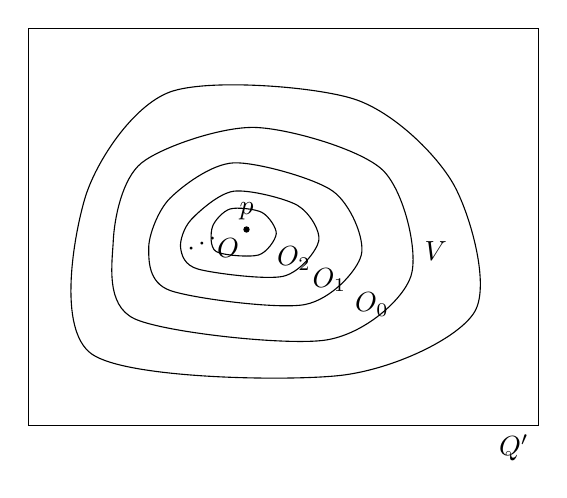
\begin{tikzpicture}[scale=0.9]
  % the 2\pi cube Q'
  \draw (0,0) rectangle (7.2,5.6);
  \node[below left] at (7.2,0) {$Q'$};
  % V
  \draw plot [smooth cycle] coordinates {(0.9,1.0) (4.4,0.7) (6.3,1.6) (6.0,3.4) (4.6,4.6) (2.0,4.7) (0.8,3.2)};
  \node at (5.75,2.45) {$V$};
  % O_0
  \draw plot [smooth cycle] coordinates {(1.5,1.5) (4.2,1.2) (5.4,2.1) (5.0,3.6) (3.2,4.2) (1.6,3.7) (1.2,2.6)};
  \node at (4.85,1.7) {$O_0$};
  % O_1
  \draw plot [smooth cycle] coordinates {(2.0,1.9) (3.9,1.7) (4.7,2.4) (4.3,3.3) (2.9,3.7) (2.0,3.2) (1.7,2.5)};
  \node at (4.25,2.05) {$O_1$};
  % O_2
  \draw plot [smooth cycle] coordinates {(2.4,2.2) (3.6,2.1) (4.1,2.6) (3.8,3.1) (2.9,3.3) (2.3,2.9) (2.15,2.5)};
  \node at (3.75,2.35) {$O_2$};
  % dots for O_3, O_4, ...
  \node at (2.6,2.62) {$\cdot$};
  \node at (2.45,2.55) {$\cdot$};
  \node at (2.3,2.48) {$\cdot$};
  % O
  \draw plot [smooth cycle] coordinates {(2.65,2.45) (3.25,2.4) (3.5,2.7) (3.3,3.0) (2.85,3.05) (2.6,2.8)};
  \node at (2.82,2.5) {$O$};
  % p
  \fill (3.08,2.76) circle (0.045);
  \node[above] at (3.08,2.76) {$p$};
\end{tikzpicture}
\end{center}

of neighborhoods $O_n$ of $p$ such that $\overline{O} \subset O_n$ and $\overline{O_n} \subset O_{n-1}$ for each $n=1,2,\ldots$. For each integer $n\geq1$, choose a $C^\infty$ function $\omega_n$ which is identically equal to 1 on $O_n$, has values between 0 and 1, and has support in $O_{n-1}$. Let


\begin{equation}
\tag{9}\label{eq:6.32:9}
v_{1}=\omega_{1}\tilde{u}\in H_{0}.
\end{equation}

Then

\begin{equation}
\tag{10}\label{eq:6.32:10}
\tilde{L}v_{1}=\tilde{L}\omega_{1}\tilde{u}=\omega_{1}\tilde{L}\tilde{u}+M_{1}\tilde{u},
\end{equation}

where

\begin{equation}
\tag{11}\label{eq:6.32:11}
M_{1}=\tilde{L}\omega_{1}-\omega_{1}\tilde{L}.
\end{equation}

In order to apply 6.30, we must first determine to which Sobolev space the right-hand side of (10) belongs.

First, we claim that


\begin{equation}
\tag{12}\label{eq:6.32:12}
\omega_{1}\tilde{L}\tilde{u}=\omega_{1}f,
\end{equation}

from which it follows that  $ \omega_1\tilde{L}\tilde{u} \in C_0^\infty(O_0) $ and thus belongs to  $ H_s $ for each  $ s $. Now both sides of (12) belong to some  $ H_s $, and it follows from \hyperref[thm:6.18]{6.18(f)} that for (12) to hold, it is sufficient to prove that

\begin{equation}
\tag{13}\label{eq:6.32:13}
\langle\omega_{1}\tilde{L}\tilde{u}-\omega_{1}f,\varphi\rangle_{0}=0
\end{equation}

for all  $ \varphi \in \mathcal{P} $. We compute, using (7), (8), \eqref{eq:6.18:9}, and \eqref{eq:6.31:2}:

\[
\begin{aligned}{\langle\omega_{1}\tilde{L}\tilde{u}-\omega_{1}f,\varphi\rangle_{0}}&{{}=\langle\omega_{1}\tilde{L}\tilde{u},\varphi\rangle_{0}-\langle\omega_{1}f,\varphi\rangle_{0}}\\ {}&{{}=\langle\tilde{L}\tilde{u},\omega_{1}\varphi\rangle_{0}-\langle f,\omega_{1}\varphi\rangle_{0}}\\ {}&{{}=\langle\tilde{u},L^{*}\omega_{1}\varphi\rangle_{0}-\tilde{l}(L^{*}\omega_{1}\varphi)}\\ {}&{{}=\tilde{l}(L^{*}\omega_{1}\varphi)-\tilde{l}(L^{*}\omega_{1}\varphi)=0.}\\ \end{aligned}
\]

Thus (12) holds. Now since $L$ (and hence $\tilde{L}$) is an operator of order 2, then $M_1$ is of order 1; hence $M_1\tilde{u} \in H_{-1}$. Thus the right-hand side of (10) belongs to $H_{-1}$. It follows from the periodic regularity \hyperref[thm:6.30]{theorem 6.30} that $v_1 \in H_1$. Now we let

\begin{equation}
\tag{14}\label{eq:6.32:14}
v_{2}=\omega_{2}\tilde{u}.
\end{equation}

Then

\begin{equation}
\tag{15}\label{eq:6.32:15}
\tilde{L}v_{2}=\omega_{2}\tilde{L}\tilde{u}+M_{2}\tilde{u}=\omega_{2}\tilde{L}\tilde{u}+M_{2}v_{1},
\end{equation}

where the last equality follows from \hyperref[thm:6.31]{6.31(4)} since  $ M_2 = \tilde{L}\omega_2 - \omega_2\tilde{L} $ has support in  $ O_1 $ and  $ \tilde{u} = v_1 $ on  $ O_1 $. Now, arguing as before, we see that the right-hand side of (15) lies in  $ H_0 $. Thus by 6.30,  $ v_2 \in H_2 $. Continuing in the same manner, we obtain

\begin{equation}
\tag{16}\label{eq:6.32:16}
v_{n}=\omega_{n}\tilde{u}\quad\text{with }v_{n}\in H_{n}.
\end{equation}

Finally, let $W_p$ be an open neighborhood of $p$ with $\overline{W}_p \subset O$, and let $\omega$ be identically 1 on $W_p$ with values between 0 and 1, and with support in $O$. Then $\omega\tilde{u} = \omega\omega_n\tilde{u}$ for each $n$; and so by (16), $\omega\tilde{u} \in H_n$ for every $n$. By the corollary to the Sobolev \hyperref[thm:6.22]{lemma 6.22}, $\omega\tilde{u}$ represents a $C^\infty$ function $u \in \mathcal{P}$. Now if $t \in C_0^\infty(W_p)$, then \index{Sobolev lemma}

\[
\begin{aligned}{l(t)}&{{}=\tilde{l}(t)=\langle\tilde{u},t\rangle_{0}=\langle\tilde{u},\omega t\rangle_{0}}\\ {}&{{}=\langle\omega\tilde{u},t\rangle_{0}=\langle u,t\rangle,}\\ \end{aligned}
\]

and (5) is proved. Except for a proof of the fact that $L$ is elliptic, this completes the proof of \hyperref[thm:6.5]{Theorem 6.5}.

\warnernumber{33}
\discuss{6.33}{Proof of \hyperref[thm:6.6]{Theorem 6.6}}\label{thm:6.33} It suffices to show that if $m \in M$, then there is some neighborhood of $m$ such that if $\varphi$ is any $C^\infty$ function on $M$ with support in that neighborhood, then $\{\varphi\alpha_n\}$ has a Cauchy subsequence. For then we simply cover $M$ by a finite number of such neighborhoods

and take a partition of unity $\varphi_{1},\ldots,\varphi_{N}$ subordinate to this cover. One can select a subsequence $\alpha_{n_{k}}$ such that $\varphi_{j}\alpha_{n_{k}}$ is Cauchy for each $j$. Then $\{\alpha_{n_{k}}\}$ is Cauchy for

\[
\begin{array}{r l}{\|\alpha_{n_{k}}-\alpha_{n_{l}}\|=\Big\|\sum_{j=1}^{N}\varphi_{j}(\alpha_{n_{k}}-\alpha_{n_{l}})\Big\|}&{\leq\quad\underset{j=1}{\overset{N}{\sum}}\|\varphi_{j}\alpha_{n_{k}}-\varphi_{j}\alpha_{n_{l}}\|.}\end{array}
\]

We reduce the problem to Euclidean space by choosing a coordinate neighborhood of $m$ with $m$ going to $p \in \mathbb{R}^n$. We continue with the notation and setup as developed in 6.31 and 6.32; in particular, the norm on $M$ and the corresponding induced norm on $C_0^\infty$ will now be denoted by $\|\cdot\|'$. Let $\varphi$ be a real-valued $C^\infty$ function with support in $O_0$. It suffices to show that the sequence $\{\varphi\alpha_{n}\}$ of elements of $\mathcal{P}$ has a Cauchy subsequence $\{\varphi\alpha_{n_{k}}\}$ in the 0-norm, since the 0-norm and the $L_2$-norm agree on $C_0^\infty(O_0)$, and the $L_2$-norm and the norm $\|\cdot\|'$ are equivalent on $C_0^\infty(O_0)$. According to the Rellich \hyperref[thm:6.23]{lemma 6.23}, in order to prove that $\{\varphi_{\alpha_n}\}$ has a Cauchy subsequence in the 0-norm, it is sufficient to show that the sequence is bounded in $H_1$. It follows from the Fundamental Inequality that

\begin{equation}
\tag{1}\label{eq:6.33:1}
\begin{aligned}{\|\varphi\alpha_{n}\|_{1}}&{{}\leq\mathrm{const}\left(\|\tilde{L}\varphi\alpha_{n}\|_{-1}+\|\varphi\alpha_{n}\|_{-1}\right)}\\ {}&{{}=\mathrm{const}\left(\|L\varphi\alpha_{n}\|_{-1}+\|\varphi\alpha_{n}\|_{-1}\right)}\\ {}&{{}\leq\mathrm{const}\|\varphi L\alpha_{n}\|_{-1}+\mathrm{const}\|(L\varphi-\varphi L)\alpha_{n}\|_{-1}+\mathrm{const}\|\varphi\alpha_{n}\|_{-1}.}\\ \end{aligned}
\end{equation}

Now

\begin{equation}
\tag{2}\label{eq:6.33:2}
\begin{aligned}{\|\varphi L\alpha_{n}\|_{-1}}&{{}\leq\|\varphi L\alpha_{n}\|_{0}=\|\varphi L\alpha_{n}\|}\\ {}&{{}\leq\mathrm{const}\|\varphi L\alpha_{n}\|^{\prime}\leq\mathrm{const}\|L\alpha_{n}\|^{\prime}\leq\mathrm{const}\|\Delta\alpha_{n}\|^{\prime}.}\\ \end{aligned}
\end{equation}

Let  $ \tau $ be a  $ C^{\infty} $ function with values between 0 and 1 which equals 1 on $O_{0}$ and has support in $V$. Then

\[
(L\varphi-\varphi L)\alpha_{n}=(L\varphi-\varphi L)(\tau\alpha_{n}),
\]

so that

\begin{equation}
\tag{3}\label{eq:6.33:3}
\begin{aligned}{\|(L\varphi-\varphi L)\alpha_{n}\|_{-1}}&{{}=\|(L\varphi-\varphi L)(\tau\alpha_{n})\|_{-1}}\\ {}&{{}\leq\mathrm{const}\|\tau\alpha_{n}\|_{0}=\mathrm{const}\|\tau\alpha_{n}\|}\\ {}&{{}\leq\mathrm{const}\|\tau\alpha_{n}\|^{\prime}\leq\mathrm{const}\|\alpha_{n}\|^{\prime}.}\\ \end{aligned}
\end{equation}

Finally,

\begin{equation}
\tag{4}\label{eq:6.33:4}
\|\varphi\alpha_{n}\|_{-1}\leq\|\varphi\alpha_{n}\|_{0}=\|\varphi\alpha_{n}\|\leq\mathrm{const}\|\varphi\alpha_{n}\|'\leq\mathrm{const}\|\alpha_{n}\|'.
\end{equation}

So from (1), (2), (3), and (4) we obtain

\begin{equation}
\tag{5}\label{eq:6.33:5}
\|\varphi\alpha_{n}\|_{1}\leq\mathrm{const}\left(\|\Delta\alpha_{n}\|^{\prime}+\|\alpha_{n}\|^{\prime}\right).
\end{equation}

But by assumption $\|\Delta\alpha_n\|'$ and $\|\alpha_n\|'$ are bounded. Therefore, the sequence $\{\varphi\alpha_n\}$ is bounded in $H_1$, and the proof of \hyperref[thm:6.6]{Theorem 6.6} is complete (assuming the ellipticity of $L$).

\section{Ellipticity of the Laplace-Beltrami Operator}


\warnernumber{34}
\begin{remarks}\label{thm:6.34}
We shall make use of the following observation. Let $U$, $V$, and $W$ be finite dimensional inner product spaces, and suppose that

\[
U \xrightarrow{A} V \xrightarrow{B} W
\]

is exact. Let $A^{*}\colon V\to U$ and $B^{*}\colon W\to V$ be the adjoints of $A$ and $B$ respectively. Then $B^{*}B+AA^{*}$ is an isomorphism on $V$. For let $v$ be a non-zero element of $V$. We need only show that $(B^{*}B+AA^{*})v\neq0$. Now

\[
\langle(B^{*}B+A A^{*})v,v\rangle=\langle B v,B v\rangle+\langle A^{*}v,A^{*}v\rangle.
\]

If $Bv \neq 0$, then $(B^*B + AA^*)v \neq 0$. If $Bv = 0$, then by the exactness, $v$ lies in the image of $A$. But $A^*$ is injective on the image of $A$. Thus $A^*v \neq 0$, which implies that $(B^*B + AA^*)v \neq 0$.

We shall apply this to the special case in which $U$, $V$, and $W$ are $\Lambda_{p-1}(M_{m}^{*}), \Lambda_{p}(M_{m}^{*})$, and $\Lambda_{p+1}(M_{m}^{*})$ respectively, with the inner products

\[
\langle\omega,\tau\rangle=\ast(\omega\wedge\ast\tau),
\]

and with $A$ and $B$ both left exterior multiplication by $\xi \in M_{m}^{*}$:

\begin{equation}
\tag{1}\label{eq:6.34:1}
\Lambda_{p-1}(M_{m}^{*})\xrightarrow{\xi}\Lambda_{p}(M_{m}^{*})\xrightarrow{\xi}\Lambda_{p+1}(M_{m}^{*}).
\end{equation}

According to Exercise 15 of Chapter 2, the sequence (1) is exact; and according to Exercise 14 of Chapter 2, the adjoint of  $ \xi\colon \Lambda_{p}(M_{m}^{*})\to\Lambda_{p+1}(M_{m}^{*}) $ is

\begin{equation}
\tag{2}\label{eq:6.34:2}
(-1)^{n p}*{\xi}*:\:\Lambda_{p+1}(M_{m}^{*})\to\Lambda_{p}(M_{m}^{*}).
\end{equation}

Thus it follows from the above remarks that

\begin{equation}
\tag{3}\label{eq:6.34:3}
(-1)^{n p}{*}\xi{*}\xi+(-1)^{n(p-1)}\xi{*}\xi{*}
\end{equation}

is an isomorphism on $\Lambda_{p}(M_{m}^{*})$.

\end{remarks}

\warnernumber{35}
\discuss{6.35}{The Laplacian is Elliptic}\label{thm:6.35} In order to complete the proofs of Theorems 6.5 and 6.6, we need to prove that the operator $L$ of 6.32 induced on Euclidean space by the Laplace-Beltrami operator $\Delta$ via a coordinate system is elliptic. Proving this, according to \eqref{eq:6.28:2}, is equivalent to showing that for each $m \in M$,

\begin{equation}
\tag{1}\label{eq:6.35:1}
\Delta(\varphi^{2}\alpha)(m)\neq0
\end{equation}

for each smooth form $\alpha$ such that $\alpha(m) \neq 0$ and for each $C^\infty$ function $\varphi$ on $M$ such that $\varphi(m) = 0$ but $d\varphi(m) \neq 0$. Assume that $\alpha$ is a $p$-form, and let $0 \neq d\varphi = \xi \in M_m^*$. Recall that

\[
\Delta=(-1)^{n(p+1)+1}d{\ast}d{\ast}+(-1)^{np+1}{\ast}d{\ast}d.
\]

We compute the left-hand side of (1), keeping in mind at each stage that  $ \varphi(m) = 0 $. Thus

\[
\begin{aligned}{d{*}d{*}(\varphi^{2}\alpha)(m)}&{{}=\big(d{*}d(\varphi^{2}){*}\alpha\big)(m)=\big(2d{*}\varphi(d\varphi){*}\alpha\big)(m)}\\ {}&{{}=\big(2(d\varphi){*}(d\varphi){*}\alpha\big)(m)=2\xi{*}\xi{*}\big(\alpha(m)\big).}\\ \end{aligned}
\]

Similarly,

\[
*d*d(\varphi^{2}\alpha)(m)=2*\xi*\xi\bigl(\alpha(m)\bigr).
\]

Thus

\[
\Delta(\varphi^{2}\alpha)(m)=-2[(-1)^{n p}\ast\xi\ast\xi+(-1)^{n(p-1)}\xi\ast\xi\ast]\bigl(\alpha(m)\bigr),
\]

which is not zero, according to \eqref{eq:6.34:3}. Hence $\Delta$ is elliptic, and the proof of the Hodge theorem is at last complete.

\warnernumber{36}
\begin{remarks}\label{thm:6.36}
We have seen that for each $\xi$ in $M_m^*$ there is a well-defined linear transformation $\sigma_\Delta(\xi)$ on $\Lambda_p(M_m^*)$ defined by

\begin{equation}
\tag{1}\label{eq:6.36:1}
\sigma_{\Delta}(\xi)(v)=\Delta(\varphi^{2}\alpha)(m),
\end{equation}

where  $ v \in \Lambda_p(M_m^*) $, where  $ \alpha $ is any  $ p $-form such that  $ \alpha(m) = v $, and where  $ \varphi $ is any  $ C^\infty $ function such that  $ \varphi(m) = 0 $ and  $ d\varphi(m) = \xi $. This linear transformation  $ \sigma_\Delta(\xi) $ is known as the symbol of the operator  $ \Delta $. The ellipticity of all the operators  $ L $ on  $ \mathbb{R}^n $ obtained from  $ \Delta $ via coordinate systems is equivalent to the property that the symbol  $ \sigma_\Delta(\xi) $ is an isomorphism at each point  $ m $ for each non-zero  $ \xi \in M_m^* $. Our computations in 6.35 contain a proof of the fact that the symbol of the exterior derivative operator  $ d $, namely  $ \sigma_d(\xi): \Lambda(M_m^*) \to \Lambda(M_m^*) $, is simply left exterior multiplication by  $ \xi $; whereas the symbol of the adjoint  $ \delta $ of  $ d $ is the adjoint of left exterior multiplication by  $ \xi $. In the theory of general partial differential operators on vector bundles over  $ M $, ellipticity is defined, as above, in terms of the symbol. \index{Symbol of a differential operator}

\end{remarks}

\section{Exercises}

\begin{problemset}

\item Prove that $*\Delta = \Delta*$.

\item (a) Prove that the Green's operator $G$ is a bounded linear operator.

(b) Prove that $G$ is self-adjoint on $(H^{p})^{\perp}$.

(c) Prove that G takes bounded sequences into sequences with Cauchy subsequences.

\item By using an integral test, prove that the series  $ \sum(1 + |\xi|^{2})^{-k} $, where  $ \xi $ ranges over all  $ n $-tuples of integers  $ (\xi_1, \ldots, \xi_n) $, converges for  $ k \geq [n/2] + 1 $. (Hint: Induct on  $ n $, and evaluate the appropriate integrals in terms of spherical coordinates.)

\item Prove in detail the inequality \eqref{eq:6.16:15}.

\item Establish the existence of the matrix $A$ of \eqref{eq:6.32:2} together with its stated properties.

\item Derive explicit formulas for $d, \ast, \delta$, and $\Delta$ in Euclidean space. In particular, show that if

\[
\alpha=\sum_{i_{1}<\cdots<i_{p}}\alpha_{I}\;d x_{i_{1}}\wedge\cdots\wedge d x_{i_{p}},
\]

then

\[
\Delta\alpha=(-1)\sum_{i_{1}<\cdots<i_{p}}\left(\sum_{i=1}^{n}\frac{\partial^{2}\alpha_{I}}{\partial x_{i}^{2}}\right)\;d x_{i_{1}}\wedge\cdots\wedge d x_{i_{p}}.
\]

\item Let $\varphi$ belong to the  $ C^{\infty} $ periodic functions  $ \mathcal{P} $ on the plane. Prove that

\[
\left\|\frac{\partial^{2}\varphi}{\partial x\,\partial y}\right\|\leq\frac{1}{2}\left\|\Delta\varphi\right\|.
\]

\item The Rellich \hyperref[thm:6.23]{lemma 6.23} says that the natural injection $i: H_{t} \to H_{s}$ for $s < t$ is a compact operator; that is, it takes bounded sequences into sequences with convergent subsequences. An analogous example of this phenomenon is the following. Let $C$ denote the Banach space of periodic continuous functions on the real line, say with period $2\pi$, and with norm the sup norm $\|\cdot\|_{\infty}$. Let $C^{1}$ be the subset of $C$ consisting of functions with continuous first derivative. As a norm for $C^{1}$ we take

\[
\left\|f\right\|=\left\|f\right\|_{\infty}+\left\|\frac{d f}{d x}\right\|_{\infty}.
\]

Use the Arzelà-Ascoli theorem [27, p. 126] to prove that the natural injection $i\colon C^{1}\to C$ is a compact operator.

\item We shall consider a number of elliptic equations of the form $Lu = f$ on the real line. In each case, $f$ will be smooth and periodic of period 1, and we look for solutions $u$ also periodic of period 1. This restriction to periodic functions makes this in essence a problem on a compact space, the unit circle. We let $u' = du/dx$. etc.

(a)  $ u' = f $. This is the simplest example of an elliptic operator which exhibits all of the essential ingredients of the theory. What is the formal adjoint of this differential operator? Show that there is a solution u (periodic) if and only if f is orthogonal to the kernel of this adjoint. \index{Elliptic equations, simple examples}

(b)  $ u^{\prime}-u=f $. What is the kernel (in the periodic functions) in this case? What are the necessary and sufficient conditions on f for there to exist a periodic solution?

(c) $u'' = f$. Show that this operator is formally self-adjoint. Show that there is a periodic solution if and only if $f$ is orthogonal to the kernel; and using the fact that

\[
\int_{0}^{x}\left(\int_{0}^{t}f(s)\,ds\right)dt=\int_{0}^{x}f(s)\left(\int_{s}^{x}dt\right)ds,
\]

show that the unique solution orthogonal to the kernel is

\[
\begin{aligned}{u(x)=}&{{}\int_{0}^{x}t(x-1)f(t)\,dt+\int_{x}^{1}x(t-1)f(t)\,dt}\\ {}&{{}+\frac{1}{2}\int_{0}^{1}t(t-1)f(t)\,dt.}\\ \end{aligned}
\]

This explicitly exhibits the Green's operator for this case.

(d) $u'' + \pi^2 u = f$. Show that this operator is formally self-adjoint. What is its kernel? Derive an explicit formula for the solution u, and show that u is periodic if and only if f is orthogonal to the kernel.

\item In \hyperref[thm:6.11]{Theorem 6.11} we used the fact that the Green's operator commutes with $d$ in proving that each closed form on a compact orientable Riemannian manifold differs from a harmonic form by an exact form. Give a proof of this result directly from the Hodge decomposition theorem without using the Green's operator.

\item A \emph{periodic distribution} $l$ is a linear functional on $\mathcal{P}$ for which there exists some integer $k \geq 0$ and a positive constant $c$ such that

\begin{equation}
|l(\varphi)|\leq c\sum_{|\alpha|\leq k}\|D^{\alpha}\varphi\|_{\infty}
\end{equation}

for all $\varphi \in \mathcal{P}$. Prove that if $l$ is a periodic distribution, then there is an element $u \in H_{-\infty}$ such that

\begin{equation}
l(\varphi)=\langle u,\varphi\rangle_{0}
\end{equation}

for all $\varphi \in \mathcal{P}$. Conversely show that every element of $H_{-\infty}$ determines a periodic distribution via (2).

\item Let $\alpha$ and $\beta$ be n-forms on a compact oriented manifold  $ M^n $ such that  $ \int_M \alpha = \int_M \beta $. Prove that  $ \alpha $ and  $ \beta $ differ by an exact form.

\item Show that \hyperref[thm:6.6]{Theorem 6.6} cannot be strengthened to the assertion of the existence of a subsequence which is convergent in  $ E^{p}(M) $.

\item One should observe that in the course of proving \hyperref[thm:6.5]{Theorem 6.5} we have proved the following regularity theorem. Let $L$ be an elliptic operator on $C^\infty$ (the complex $m$-space valued smooth functions on $\mathbb{R}^n$). Suppose that $u$ is sufficiently differentiable for $Lu$ to make sense, and suppose that $Lu = f$ where $f \in C^\infty$. Then $u \in C^\infty$.

In fact, we have proved more—every weak solution $l$ is smooth. Precisely: Let $l$ be a linear functional on $C_0^\infty$ which is bounded on $C_0^\infty(V)$ whenever $\overline{V}$ is compact, and which satisfies $l(L^*\varphi) = \langle f, \varphi \rangle$ for every $\varphi \in C_0^\infty$. Then $l$ is smooth in the sense that there exists $u \in C^\infty$ which represents $l$; that is, $l(t) = \langle u, t \rangle$ for every $t \in C_0^\infty$. Such a smooth representative $u$ of a weak solution $l$ is an actual solution, $Lu = f$.

\item Observe that the Cauchy-Riemann operator $(\partial/\partial x) + i(\partial/\partial y)$ is elliptic. Conclude from the general theory of elliptic operators that every holomorphic function is $C^{\infty}$. Prove that every holomorphic function is a complex-valued harmonic function on the plane, and use Green's 1st identity (Exercise 5, Chapter 4) to prove that a holomorphic function with compact support must be identically zero.

\item \textbf{The Eigenvalues of the Laplacian}\quad This is an extended exercise in which the fundamental properties of the eigenfunctions and eigenvalues of the Laplacian are developed. Proofs for the more difficult parts are outlined, and in some cases are given nearly in full.

Consider the Laplace-Beltrami operator  $ \Delta $ acting on the p-forms  $ E^{p}(M) $ for some fixed p. A real number  $ \lambda $ corresponding to which there exists a not identically zero p-form u such that  $ \Delta u = \lambda u $ is called an eigenvalue of  $ \Delta $. If  $ \lambda $ is an eigenvalue, then any p-form u such that  $ \Delta u = \lambda u $ is called an eigenfunction of  $ \Delta $ corresponding to the eigenvalue  $ \lambda $. The eigenfunctions corresponding to a fixed  $ \lambda $ form a subspace of  $ E^{p}(M) $ called the eigenspace of the eigenvalue  $ \lambda $. \index{Cauchy-Riemann operator}\index{Harmonic function}

(a) Prove that the eigenvalues of  $ \Delta $ are non-negative.

(b) Prove that the eigenspaces of  $ \Delta $ are finite dimensional.

(c) Prove that the eigenvalues have no finite accumulation point.

(d) Prove that eigenfunctions corresponding to distinct eigenvalues are orthogonal.

(e) Existence. In order for the above statements to have substance we must prove that there exist eigenvalues of $\Delta$. First of all, zero is an eigenvalue if and only if there are non-trivial harmonic $p$-forms on $M$, and the corresponding eigenspace is precisely the space $H^p$ of harmonic forms. We shall now establish that $\Delta$ has a positive eigenvalue—in fact, a whole sequence of eigenvalues diverging to $+\infty$. Consider $\Delta$ to be restricted to $(H^p)^\perp$. Then we have $\Delta: (H^p)^\perp \to (H^p)^\perp$, and also we have the Green's operator $G: (H^p)^\perp \to (H^p)^\perp$, and $\Delta G\alpha = \alpha$, $G\Delta\alpha = \alpha$ for all $\alpha \in (H^p)^\perp$. Observe that the eigenvalues of $G \mid (H^p)^\perp$ are the reciprocals of the eigenvalues of $\Delta \mid (H^p)^\perp$. Let

\[
\eta=\sup_{\substack{\|\varphi\|=1\\ \varphi\in(H^{p})^{\perp}}}\|G\varphi\|.
\]

Then $\eta > 0$ and $\|G\varphi\| \leq \eta \|\varphi\|$ for every $\varphi \in (H^{p})^{\perp}$. We shall prove that $1/\eta$ is an eigenvalue of $\Delta$. Let $\{\varphi_j\} \in (H^{p})^{\perp}$ be a maximizing sequence for $\eta$; that is, $\|\varphi_j\| = 1$ and $\|G\varphi_j\| \to \eta$.

First, we claim that  $ \|G^2\varphi_j - \eta^2\varphi_j\| \to 0 $, for

\[
\begin{aligned}{\|G^{2}\varphi_{j}-\eta^{2}\varphi_{j}\|^{2}}&{{}=\|G^{2}\varphi_{j}\|^{2}-2\eta^{2}\langle G^{2}\varphi_{j},\varphi_{j}\rangle+\eta^{4}}\\ {}&{{}\leq\eta^{2}\|G\varphi_{j}\|^{2}-2\eta^{2}\|G\varphi_{j}\|^{2}+\eta^{4}\to0.}\\ \end{aligned}
\]

Second, we claim that $\|G\varphi_j - \eta\varphi_j\| \to 0$. For if we let $\psi_j = G\varphi_j - \eta\varphi_j$, then

\[
\begin{aligned}{0\leftarrow\langle\psi_{j},G^{2}\varphi_{j}-\eta^{2}\varphi_{j}\rangle}&{{}=\langle\psi_{j},G\psi_{j}+\eta\psi_{j}\rangle}\\
{}&{{}=\langle\psi_{j},G\psi_{j}\rangle+\eta\|\psi_{j}\|^{2}\geq\eta\|\psi_{j}\|^{2},}\\
\end{aligned}
\]

where we have used the fact that $\langle\psi_{j},G\psi_{j}\rangle\geq0$. (Why?) Now there is a subsequence of the $\varphi_j$, call it $\{\varphi_j\}$, such that $\{G\varphi_j\}$ is Cauchy. Define a linear functional $l$ on $E^p(M)$ by setting

\[
l(\beta)=\lim_{j\to\infty}\eta\langle G\varphi_{j},\beta\rangle\quad\text{for}\quad\beta\in E^{p}(M).
\]

Prove that $l$ is a non-trivial weak solution of

\[
\big(\Delta-(1/\eta)\big)u=0.
\]

From this and the fact that  $ \Delta - 1/\eta $ is elliptic, conclude that  $ \lambda = 1/\eta $ is an eigenvalue of  $ \Delta $.

(f) Existence of Other Eigenvalues. Suppose that we have eigenvalues  $ \lambda_1 \leq \lambda_2 \leq \cdots \leq \lambda_n $ and corresponding eigenfunctions  $ u_1, u_2, \ldots, u_n $ (orthonormalized) for  $ \Delta \big| (H^p)^{\perp}  $. Let  $ R_n $ be the subspace of  $ (H^p)^{\perp} $ spanned by  $ \{u_1, \ldots, u_n\} $. Observe that  $ G $ and  $ \Delta $ map  $ (H^p \oplus R_n)^{\perp} $ into itself, then define

\[
\eta_{n+1}=\sup_{\substack{\|\varphi\|=1\\ \varphi\in(H^{p}\oplus R_{n})^{\perp}}}\|G\varphi\|
\]

and proceed as in part (e) to establish that  $ \lambda_{n+1} = 1/\eta_{n+1} $ is an eigenvalue of  $ \Delta $. Clearly,  $ \lambda_{n+1} \geq \lambda_n $.

(g) $L_{2}$ Completeness. Let $\lambda_{1} \leq \lambda_{2} \leq \cdots$ be the eigenvalues of $\Delta$ on $E^{p}(M)$, where each eigenvalue is included as many times as the dimension of its eigenspace, with a corresponding orthonormalized sequence of eigenfunctions $\{u_{i}\}$. Let $\alpha \in E^{p}(M)$. Then

\[
\lim_{n\to\infty}\left\|\alpha-\sum_{i=1}^{n}\langle\alpha,u_{i}\rangle u_{i}\right\|=0.
\]

For the proof, let $k$ be the dimension of $H^p$. Then there exists $\beta \in (H^p)^\perp$ such that $G\beta = \alpha - \sum_{i=1}^{k} \langle \alpha, u_i \rangle u_i$. It follows that

\[
\left\|\alpha-\sum_{i=1}^{n}\langle\alpha,u_{i}\rangle u_{i}\right\|=\left\|G\left(\beta-\sum_{i=k+1}^{n}\langle\beta,u_{i}\rangle u_{i}\right)\right\|
\]

for $n > k$. But, by the definition of $\lambda_{n+1}$,


\begin{align*}\bigg\|G\bigg(\beta-\sum_{i=k+1}^{n}\langle\beta,u_{i}\rangle u_{i}\bigg)\bigg\|&\leq\frac{1}{\lambda_{n+1}}\bigg\|\beta-\sum_{i=k+1}^{n}\langle\beta,u_{i}\rangle u_{i}\bigg\|\\&\leq\frac{1}{\lambda_{n+1}}\|\beta\|\to0\quad as\quad n\to\infty.\end{align*}


(h) Uniform Completeness. The uniform norm  $ \|\alpha\|_{\infty} $ is defined on  $ E^{p}(M) $ by

\[
\|\alpha\|_{\infty}=\sup_{m\in M}\left(*(\alpha\wedge*\alpha)(m)\right)^{1/2}.
\]

From the Sobolev inequality \hyperref[thm:6.22]{6.22(1)} and the compactness of $M$, one can conclude that there exists a large enough integer $k$ and a constant $c > 0$ such that

\[
\|\alpha\|_{\infty}\leq c\|(1+\Delta)^{k}\alpha\|
\]

for every $\alpha \in E^p(M)$. Let $\alpha \in E^p(M)$, and let $P_n(\alpha) = \sum_{i=1}^{n} \langle \alpha, u_i \rangle u_i$, where we are continuing with the notation of part (g). Now $\Delta P_n = P_n \Delta$, so that

\[
\begin{aligned}{\|\alpha-P_{n}(\alpha)\|_{\infty}}&{{}\leq c\left\|(1+\Delta)^{k}[\alpha-P_{n}(\alpha)]\right\|}\\ {}&{{}=\|\varphi-P_{n}\varphi\|\to0,}\\ \end{aligned}
\]

where  $ \varphi = (1 + \Delta)^{k}\alpha $.

\item We define the operator  $ \Delta^2 \colon E^p(M) \to E^p(M) $ by  $ \Delta^2(\alpha) = \Delta(\Delta\alpha) $. Discuss the solvability of  $ \Delta^2\alpha = \beta $.

\item Consider the operator

\[
L=\sum_{i,j=1}^{n}a_{ij}\frac{\partial^{2}}{\partial x_{i}\partial x_{j}}+\sum_{i=1}^{n}b_{i}\frac{\partial}{\partial x_{i}}+c
\]

acting on $C^{2}(\mathbb{R}^{n})$. Show that there is no loss of generality in assuming that $a_{ij}=a_{ji}$, and prove that $L$ is elliptic at a point $x$ if and only if the matrix $(a_{ij}(x))$ is (positive or negative) definite. In particular, show that the wave equation \index{Wave equation}

\[
\Box u=\frac{\partial^{2}u}{\partial x^{2}}-\frac{\partial^{2}u}{\partial y^{2}}=f
\]

is not elliptic, and give an example where

\[
\Box u=f\in C^{\infty}\quad\text{but}\quad u\notin C^{\infty}.
\]

\item Consider $\Delta\colon E^p(M)\to E^p(M)$. Prove that if $\lambda$ is the minimum eigenvalue of $\Delta$, and if $c>-\lambda$, then $(\Delta+c)\alpha=\beta$ can be solved for every $\beta\in E^p(M)$.

\item \textbf{The Peter-Weyl Theorem}\quad The representative ring of a compact Lie group $G$ is the ring generated over the complex numbers by the set of all continuous functions $f$ for which there is a continuous homomorphism $\rho\colon G \to Gl(n,\mathbb{C})$ for some $n$ such that $f = \rho_{ij}$ for some choice of $i$ and $j$. The Peter-Weyl theorem states that the representative ring is dense in the space of complex-valued continuous functions on $G$ in the uniform norm. That is, if $g$ is a complex-valued continuous function on $G$, and if $\varepsilon > 0$ is given, then there is a function $f$ in the representative ring such that $|f(\sigma) - g(\sigma)| < \varepsilon$ for all $\sigma \in G$. We outline a proof of this theorem which is based on the uniform completeness of the eigenfunctions of the Laplacian. One can choose a Riemannian structure on $G$ such that each of the diffeomorphisms $l_\sigma$ for $\sigma \in G$ (left translation by $\sigma$) is an isometry (that is, $\langle v, w \rangle_\tau = \langle dl_\sigma v, dl_\sigma w \rangle_{\sigma\tau}$ for all $\tau \in G$ and all $v, w \in G_\tau$). Since the $C^\infty$ functions are dense in the space of continuous functions in the uniform norm, and since by Exercise 16(h) the direct sum of the eigenspaces of the Laplacian is dense in the space of $C^\infty$ functions in the uniform norm, it suffices for the Peter-Weyl theorem to prove that each eigenfunction of the Laplacian $\Delta: C^\infty(G) \to C^\infty(G)$ belongs to the representative ring.

Now, $G$ acts on the $C^{\infty}$ functions on $G$ by \index{Peter-Weyl theorem}

\[
\sigma(f)=f\circ l_{\sigma}\quad\text{for }\sigma\in G.
\]

Prove that since the $l_{\sigma}$ are isometries, this action commutes with the Laplacian:

\[
\Delta(f\circ l_{\sigma})=(\Delta f)\circ l_{\sigma}\qquad(\sigma\in G).
\]

Let $V_\lambda$ be the (finite dimensional) eigenspace associated with the eigenvalue $\lambda$ of $\Delta\colon C^\infty(G) \to C^\infty(G)$. Prove that the action of $G$ leaves $V_\lambda$ invariant. Then let $\varphi_1, \ldots, \varphi_n$ be a basis of $V_\lambda$, and let

\[
\sigma(\varphi_{i})=\sum_{j}g_{i j}(\sigma)\varphi_{j}.
\]

Then $\sigma \mapsto \{g_{ij}(\sigma)\}$ is a homomorphism of $G \to Gl(n, \mathbb{R})$. Prove that this homomorphism is continuous. Then observe that

\[
\varphi_{i}(\sigma)=\varphi_{i}\circ l_{\sigma}(e)=\sum_{j}g_{i j}(\sigma)\varphi_{j}(e),
\]

so that  $ \varphi_{i} $ belongs to the representative ring.

\item The reader who is familiar with the theory of vector bundles should observe that the results in this chapter on the Laplace-Beltrami operator are valid for general elliptic operators on vector bundles. We outline the statements of the results in this situation:

Let $E$ and $F$ be (real or complex) vector bundles over a compact orientable manifold $M$. Let $C^\infty(E)$ and $C^\infty(F)$ denote the vector spaces of smooth sections of $E$ and $F$ respectively. A (linear) differential operator $L$ of order $l$ from $E$ to $F$ is a linear map from $C^\infty(E)$ to $C^\infty(F)$ which when expressed in terms of local trivialization of $E$ and $F$ yields an ordinary linear partial differential operator of order $l$. The operator $L$ is elliptic if it is locally elliptic. Equivalently, ellipticity of $L$ can be defined in terms of the symbol as in 6.36. Observe that for $L$ to be elliptic, the fibre dimensions of $E$ and $F$ must be equal. Choose inner products in the fibres $E_m$ and $F_m$ which vary smoothly with $m$, and choose a Riemannian structure and an orientation on $M$ with respect to which smooth functions can be integrated over $M$. By integrating the fibre inner products over $M$, we obtain inner products on $C^\infty(E)$ and $C^\infty(F)$. Let $L: C^\infty(E) \to C^\infty(F)$ be a differential operator. Prove that $L$ has a formal adjoint $L^*: C^\infty(F) \to C^\infty(E)$. Assume that $L$ is elliptic.

(a) Prove that $\ker L$ and $\ker L^{*}$ are finite dimensional.

(b) Prove that  $ C^{\infty}(E) $ and  $ C^{\infty}(F) $ have the following orthogonal direct sum decompositions:

\[
\begin{aligned}{}&{{}C^{\infty}(F)=L\big(C^{\infty}(E)\big)\oplus\ker L^{*},}\\ {}&{{}C^{\infty}(E)=L^{*}\big(C^{\infty}(F)\big)\oplus\ker L.}\\ \end{aligned}
\]

\item Let $\varphi_n$, for $n=1,2,3,\ldots$, be a periodic $C^\infty$ function on the plane which agrees with $\log \log(1/(r+(1/n)))$ for $0 \leq r \leq \frac{1}{2}$, where $r = \sqrt{x^2 + y^2}$. Show that there is no constant $c > 0$ such that

\[
\left\|\varphi_{n}\right\|_{\infty}\leq c\left\|\varphi_{n}\right\|_{1}\qquad\text{for all }n.
\]

This shows, in the case $n=2$, that the restriction $t\geq[n/2]+1$ in Corollary (b) of the Sobolev \hyperref[thm:6.22]{lemma 6.22} is essential.

\item Let $L$ be a (linear) elliptic operator on the $C^\infty$ functions on a compact oriented Riemannian manifold $M$. Let $\gamma$ be a diffeomorphism of $M$ which preserves the volume form on $M$. We say that a $C^\infty$ function $f$ on $M$ is invariant under $\gamma$ if $f\circ\gamma=f$, and we say that the operator $L$ is invariant under $\gamma$ if $Lu\circ\gamma=L(u\circ\gamma)$ for all $C^\infty$ functions $u$ on $M$. Suppose that $L$ and $f$ are invariant under $\gamma$ and that $f$ is orthogonal to the kernel of $L^*$. Prove that there is an invariant solution $u$ of $Lu=f$.

\end{problemset}
